\listfiles
\documentclass[3p]{elsarticle}

\usepackage{lineno,hyperref}
\usepackage{amsmath} 
\usepackage{float} 
\modulolinenumbers[5]

\journal{Applied Machine Learning Course}

%%%%%%%%%%%%%%%%%%%%%%%
%% Bibliography styles
%%%%%%%%%%%%%%%%%%%%%%%
%% To change the style, put a % in front of the second line of the current style and
%% remove the % from the second line of the style you would like to use.
%%%%%%%%%%%%%%%%%%%%%%%

% Numbered
% \bibliographystyle{model1-num-names}

%% Numbered without titles
% \bibliographystyle{model1a-num-names}

%% Harvard
% \bibliographystyle{model2-names}\biboptions{authoryear}

%% Vancouver numbered
% \usepackage{numcompress}\bibliographystyle{model3-num-names}

%% Vancouver name/year
% \usepackage{numcompress}\bibliographystyle{model4-names}\biboptions{authoryear}

%% APA style
% \bibliographystyle{model5-names}\biboptions{authoryear}

%% AMA style
% \usepackage{numcompress}\bibliographystyle{model6-num-names}

%% `Elsevier LaTeX' style, distributed in TeX Live 2019
\bibliographystyle{elsarticle-num}
% \usepackage{numcompress}\bibliographystyle{elsarticle-num-names}
% \bibliographystyle{elsarticle-harv}\biboptions{authoryear}
%%%%%%%%%%%%%%%%%%%%%%%

%%%%%%%%%%%%%%%%%%%%%%%%%%%%%%%%%%%%%%%%%%%%%%%%%%%%%%%%%%%%%%%
% DO NOT EDIT ANYTHING ABOVE THIS LINE
% EXCEPT IF YOU LIKE TO USE ADDITIONAL PACKAGES
%%%%%%%%%%%%%%%%%%%%%%%%%%%%%%%%%%%%%%%%%%%%%%%%%%%%%%%%%%%%%%%



\begin{document}

\begin{frontmatter}

%%%%%%%%% TITLE
\title{Applied Machine Learning Project: TurboFan Engine Remaining Useful Life (RUL)}

%%%%%%%%% AUTHORS
\author{Roberto Cialini}
\ead{rocia24@student.sdu.dk}

\author{Jaka Škerjanc}
\ead{jaske24@student.sdu.dk}

\author{Riccardo Rossi-Erba}
\ead{riros24@student.sdu.dk}

\author{Jan Fiala}
\ead{jafia24@student.sdu.dk}

\author{Chisom Okoye}
\ead{choko23@student.sdu.dk}

%%%%%%%%% ABSTRACT
\begin{abstract}
With technological advancements, turbofan engines, essential components of aircraft, have become more complex. The complexity of turbofan engines has increased significantly with technological advancements, making effective maintenance strategies crucial. About 60\% of aircraft breakdowns involve turbofan engines, influenced by varying operating hours and conditions \cite{wei2018study}.
Traditional maintenance methods, such as corrective and preventive maintenance, are inadequate for ensuring optimal performance and reliability. This study explores Prognostics and Health Management (PHM) techniques, focusing on the prediction of the Remaining Useful Life (RUL) of turbofan engines using data-driven approaches.

The paper shows a variety of machine learning models, including Linear Regression, Elastic Net Regression, Random Forests Regression, Support Vector Machines Regression, and Neural Networks, to analyze historical sensor data and predict engine degradation. The results indicate that ensemble methods like Random Forests  and advanced models such as Support Vector Machine Regression with RBF kernel provide superior performance compared to simpler models, demonstrating higher accuracy and robustness in RUL prediction.

The findings suggest that these data-driven models can significantly enhance the reliability of maintenance strategies for turbofan engines.
\end{abstract}
\end{frontmatter}

\linenumbers


% MAIN ARTICLE GOES BELOW
%%%%%%%%%%%%%%%%%%%%%%%%%%%%%%%%%%%%%%%%%%%%%%%%%%%%%%%%%%%%%%%


%%%%%%%%% BODY TEXT
\label{Introduction}
\section{Introduction}
Turbofan engines are the backbone of modern aviation, powering the majority of commercial and military aircraft. However, these complex machines are susceptible to degradation throughout their operational lifespan, leading to significant safety concerns and increased maintenance costs. Unscheduled engine failures pose serious threats to passenger and crew safety, with the Federal Aviation Administration (FAA) reporting that engine-related issues account for approximately 25\% of all in-flight emergencies \cite{faa2022}. Reactive maintenance approaches based on fixed service intervals can be inefficient and costly, with the average cost of an unscheduled engine removal exceeding \$1.5 million \cite{iata2021}.

Traditional maintenance strategies like corrective and preventive maintenance have proven insufficient. Prognostics and Health Management (PHM), also known as condition-based or predictive maintenance, addresses these challenges by ensuring optimal system performance, preventing failures, reducing maintenance costs, and managing system health. PHM is critical in aviation, where reliability is paramount due to the severe consequences of accidents. This paper focuses on turbofan engines, the most complex and critical aircraft components, requiring high reliability and quality. Predicting Remaining Useful Life (RUL) is essential for developing cost-effective maintenance strategies and enhancing reliability.

More in detail, this paper explores the application of Machine Learning (ML) techniques for predicting the RUL of turbofan engines. By analyzing sensor data collected throughout the engine's lifecycle, including parameters such as vibration, temperature, fuel consumption, and engine speed, ML models can identify patterns and trends indicative of impending degradation. This predictive capability enables proactive maintenance strategies, allowing for interventions to be scheduled before critical failures occur.

The benefits of implementing an RUL prediction system are multifaceted. Early detection of degradation facilitates targeted maintenance actions, minimizing the risk of catastrophic failures and enhancing overall operational safety. According to the International Air Transport Association (IATA), predictive maintenance can reduce unscheduled maintenance events by up to 30\% and decrease maintenance costs by 20\% \cite{iata2023}. This paper delves into the development and evaluation of various ML algorithms for RUL prediction, using real-world engine data sets from aircraft manufacturers and engine test rigs.

RUL prediction methods are categorized into model-based, data-driven, and hybrid approaches. Model-based methods use mathematical models to describe system degradation but are costly and require expertise. Data-driven methods analyze historical sensor data to understand degradation with less expertise needed. Hybrid approaches combine both methods but have their limitations.

In our project, we utilized data-driven models to predict the RUL of turbofan engines. The models implemented include Linear Regression, Elastic Net Regression, Random Forests Regression, Support Vector Machines Regression, and Neural Networks. These models leverage historical sensor data to accurately predict engine degradation and remaining useful life. By employing these data-driven approaches, we aim to enhance prediction accuracy, reduce maintenance costs, and improve the overall reliability of turbofan engines.

The remainder of this paper is organized as follows. Section 2 reviews related work addressing the same problem. Section 3 outlines the algorithms and methods used in this study. The results are presented in Section 4. The paper concludes with a summary in Section 5, followed by a discussion of contributions in Section 6. 

\section{Related Work}

Predicting the remaining useful life (RUL) of turbofan jet engines has been extensively studied, leveraging various machine learning algorithms and datasets. Ali Alhamaly (2019)\cite{Alhamaly} explored a data-driven approach for predictive maintenance using the NASA C-MAPSS dataset, which simulates the degradation of commercial turbofan engines under various operational conditions. Alhamaly focused on preprocessing steps such as dimensionality reduction through PCA and the development of a health index to fuse sensor data, utilizing linear regression for trend analysis and exponential models for RUL prediction.

Similarly, Thakkar and Chaoui (2022)\cite{ThakkarUnnati2022} employed deep learning models, specifically Deep Layer Recurrent Neural Networks (DL-RNN), to enhance RUL prediction accuracy. Their study compared DL-RNN with other neural network architectures like Multilayer Perceptron (MLP) and Nonlinear Auto Regressive Network with Exogenous Inputs (NARX), demonstrating superior performance of DL-RNN on the C-MAPSS dataset with significantly lower error rates (MAE and RMSE) compared to the alternative models.

In another study, Liu et al. (2023)\cite{E2023} applied various machine learning algorithms to the NASA turbofan engine dataset, including linear regression, K-nearest neighbors (KNN), elastic net, random forests, support vector machines (SVM), and regression trees. Their research aimed to evaluate the effectiveness of these simpler models in RUL prediction, highlighting that ensemble methods like random forests and more sophisticated algorithms such as SVM provided competitive results compared to deep learning models.

Solis-Martin, Galan-Paez, and Borrego-Diaz \cite{Solis-Martin} even went further to develop an approach to determine the RUL of jet engines that has been considered innovative and ranked in the third place of the 2021 PHM Conference Data Challenge. The technique involves tow Deep Convolutional Neural Networks stacked on two levels. While the first is used to extract low-dimensional feature vector based on the normalized raw data as input, the second DCNN injects a list of vectors and estimates RUL for the jet engines and the results show excellent outcomes.

Most of the existing literature focuses on advanced neural network models for RUL prediction. However, in our work, we chose to stick to simpler machine learning algorithms. This decision was driven by a desire to explore the effectiveness of these more interpretable and less computationally intensive models, providing a baseline for comparison against more complex approaches.

By integrating insights from prior studies and our experimental evaluations, we aim to contribute a comparative analysis of traditional machine learning methods for RUL prediction, providing a benchmark for future research and practical implementations in the field of prognostics and health management of aircraft engines.

\section{Proposed Method}

First we conducted a thorough analysis and preprocessing of the dataset to prepare it for modeling in section 3.1. In the data pre-processing phase the initial step involves removing columns with constant values, as these do not provide useful information for predictive modeling. Next, the RUL values are capped to a specific constant value to limit the range and effectively manage outliers. Columns that do not show a significant correlation with the target variable, RUL, are dropped to reduce dimensionality and improve model performance. Additionally, sensor data is smoothed to reduce noise and enhance the signal quality, aiding in more accurate predictions.

Following data pre-processing, the cleaned data is used to train various machine learning models. The models include linear and elastic net regression, random forest regression, regression tree, support vector machine (SVM) regressor with both linear and RBF kernels. Additionally, a basic neural network model is used to capture complex patterns in the data. This is the core of the section 3.2

The trained models are evaluated using cross-validation to ensure their robustness and generalizability. Four metrics are used to measure the performance of the models\cite{MetricsArticle}:

\begin{enumerate}
    \item Mean Absolute Error (MAE): measures the average magnitude of errors in a set of predictions, without considering their direction.
    \item Mean Square Error (MSE): quantifies the error by squaring the difference between actual and predicted values.
    \item Root Mean Squared Error (RMSE): provides the square root of the average squared differences between actual and predicted values, giving a more interpretable error measure.
    \item $R^2$ Score: represents the proportion of the variance for the dependent variable that's explained by the independent variables in the model.
\end{enumerate}

Figure 1 gives an overview about the workflow.

\subsection{Project Analysis and Preprocessing}

\subsubsection{Data description}
The datasets consist of multiple multivariate time series. Each time series represents a different engine, simulating a fleet of engines of the same type. Each engine begins with varying degrees of initial wear and manufacturing variation, which are unknown to the user. These variations are considered normal and not indicative of faults. The data includes three operational settings that significantly affect engine performance, along with sensor noise contamination.

At the start of each time series, the engines operate normally, but a fault develops over time. In the training set, this fault grows until the system fails, while in the test set, the time series ends before system failure. The competition's objective is to predict the remaining operational cycles before failure in the test set, i.e., the number of cycles the engine will continue to operate after the last recorded cycle. A vector of true Remaining Useful Life (RUL) values for the test data is also provided.

The dataset is made by 26 features. Each row represents a snapshot of data taken during a single operational cycle, with each column representing a different variable. The columns correspond to the unit number, time in cycles, three operational settings, and twenty-one sensor measurements.

The dataset, labeled FD001, includes 100 train trajectories all under one condition at sea level and exhibiting one fault mode, specifically HPC (high-pressure compressor) degradation.

\begin{figure}[H]
    \centering
    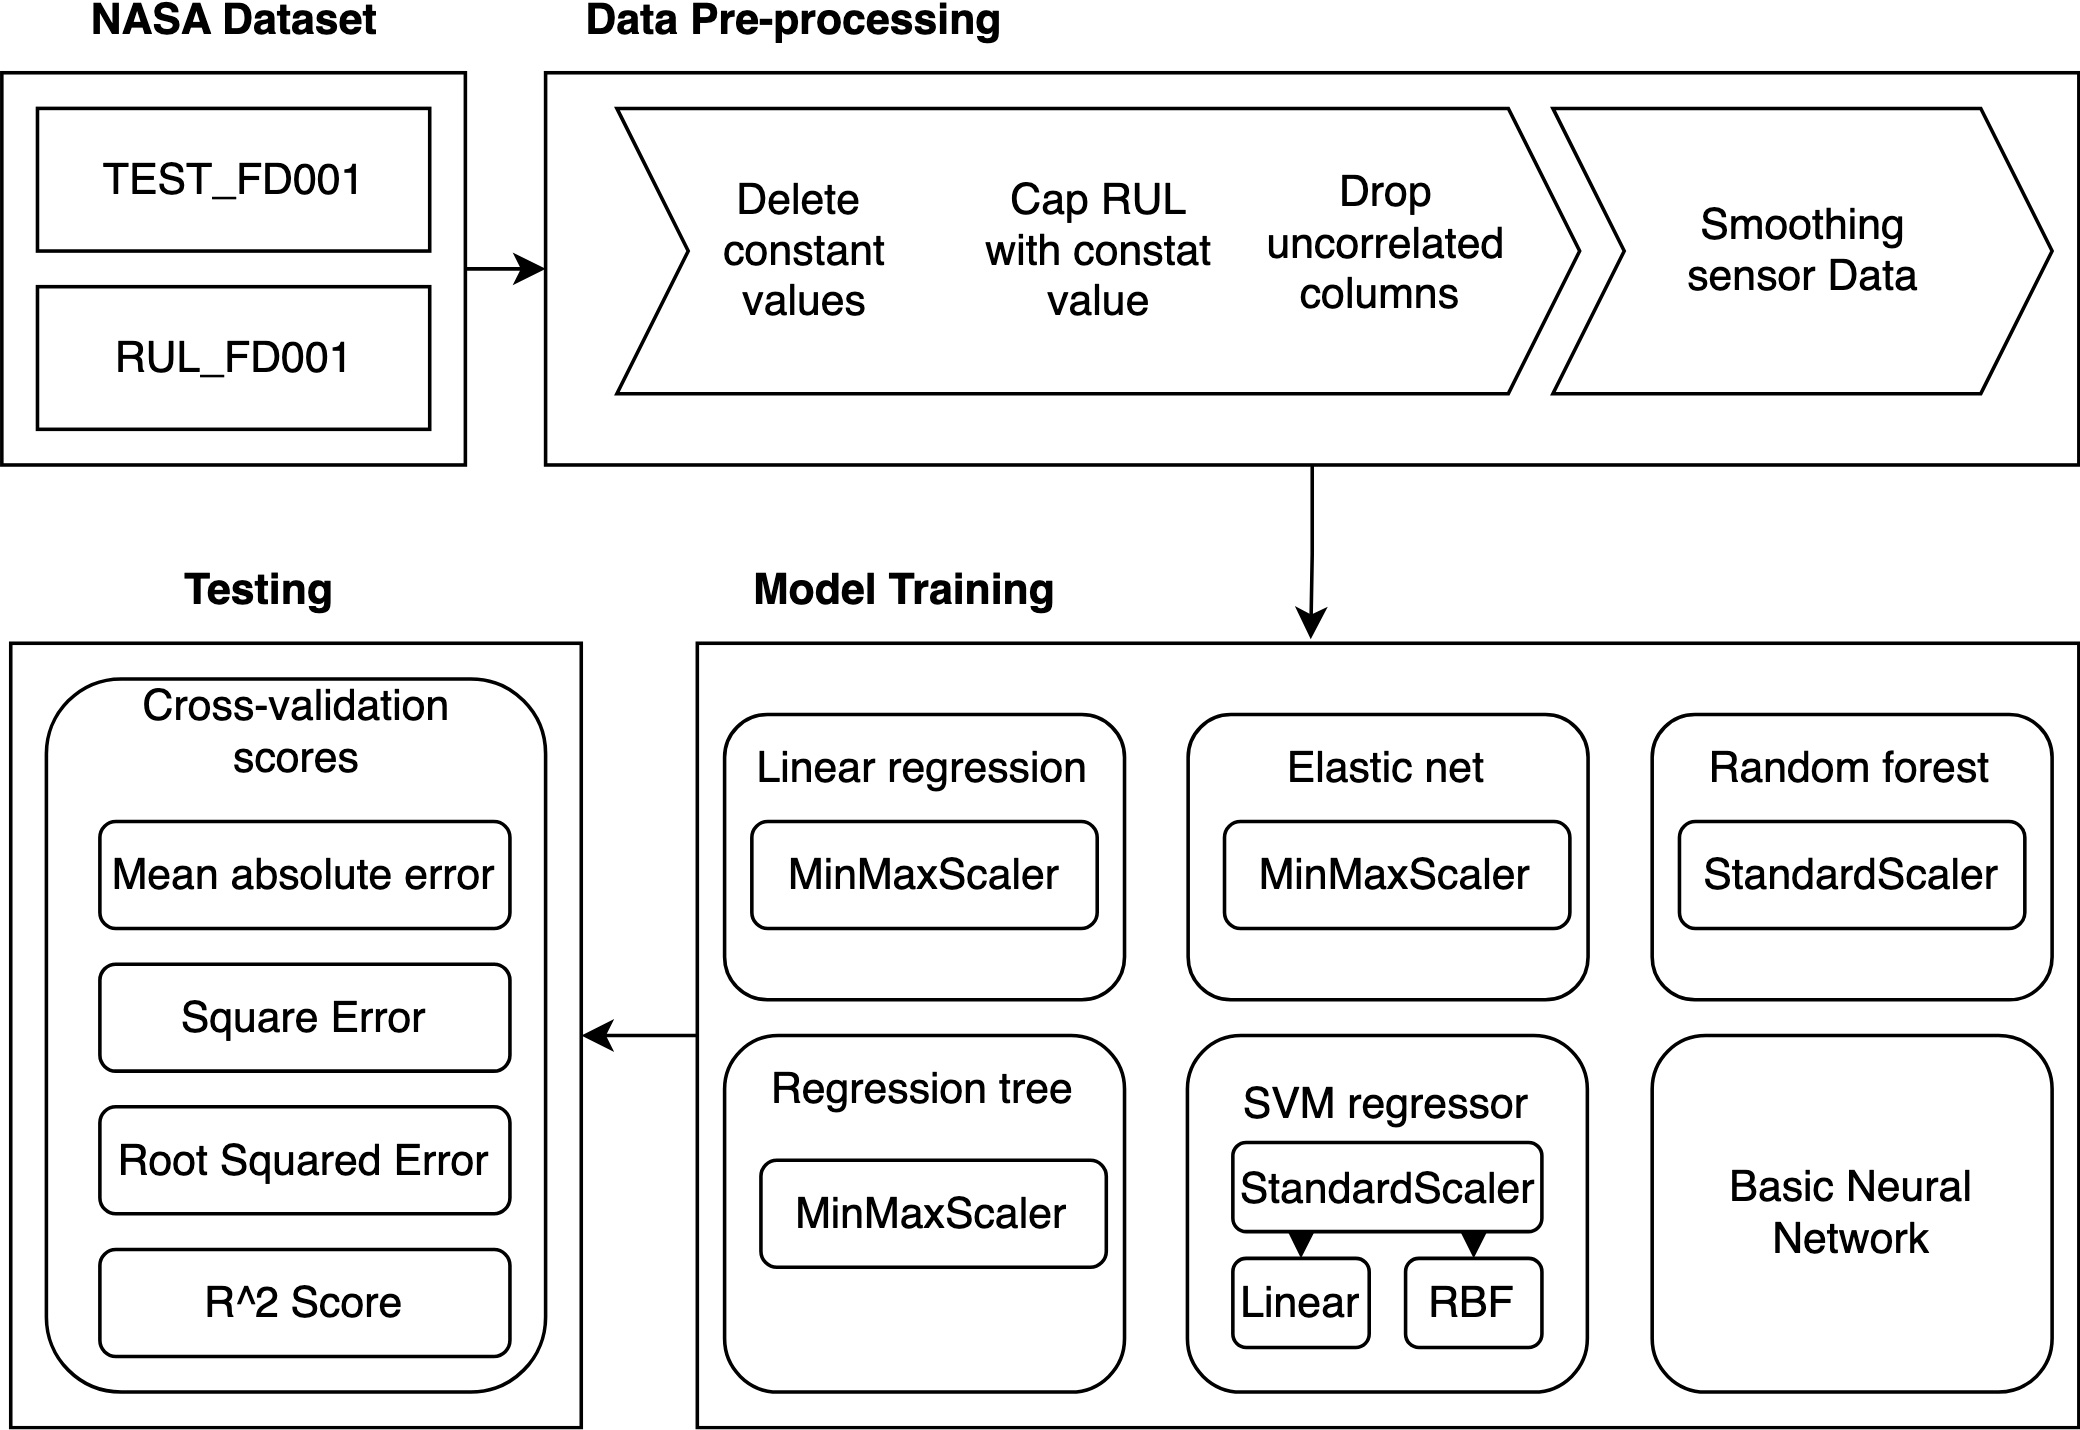
\includegraphics[width=1\textwidth]{images/aml-workflow.jpg}
    \caption{Project workflow.}
    \label{fig:diagram_architecture}
\end{figure}


\subsubsection{Data analysis}

Initially, we imported the necessary libraries and loaded the dataset. The column names were defined for better readability, which included operational settings and sensor measurements with added the RUL column, that was calculated based on the maximum cycle per engine and the current cycle.

We then provided a summary of the dataset to understand its basic statistics and computed the correlation matrix (figure \ref{fig:correlation_matrix}) to identify relationships between different variables. 

This step was crucial for feature selection, as it helped identify which features were most relevant to the RUL prediction.

To visualize the sensor data, we plotted the signals from the sensors for a subset of engines. This visualization helped us understand the patterns and trends within the sensor data, revealing significant insights into engine behavior over time.

\subsubsection{Data cleaning}
In the data cleaning phase, we identified and removed columns with constant values, as they do not contribute to the model's predictive power. Additionally, we removed columns that were not correlated with RUL, focusing only on the relevant features. This step ensured that the dataset was concise and contained only useful information for training the model.

\begin{figure}[H]
    \centering
    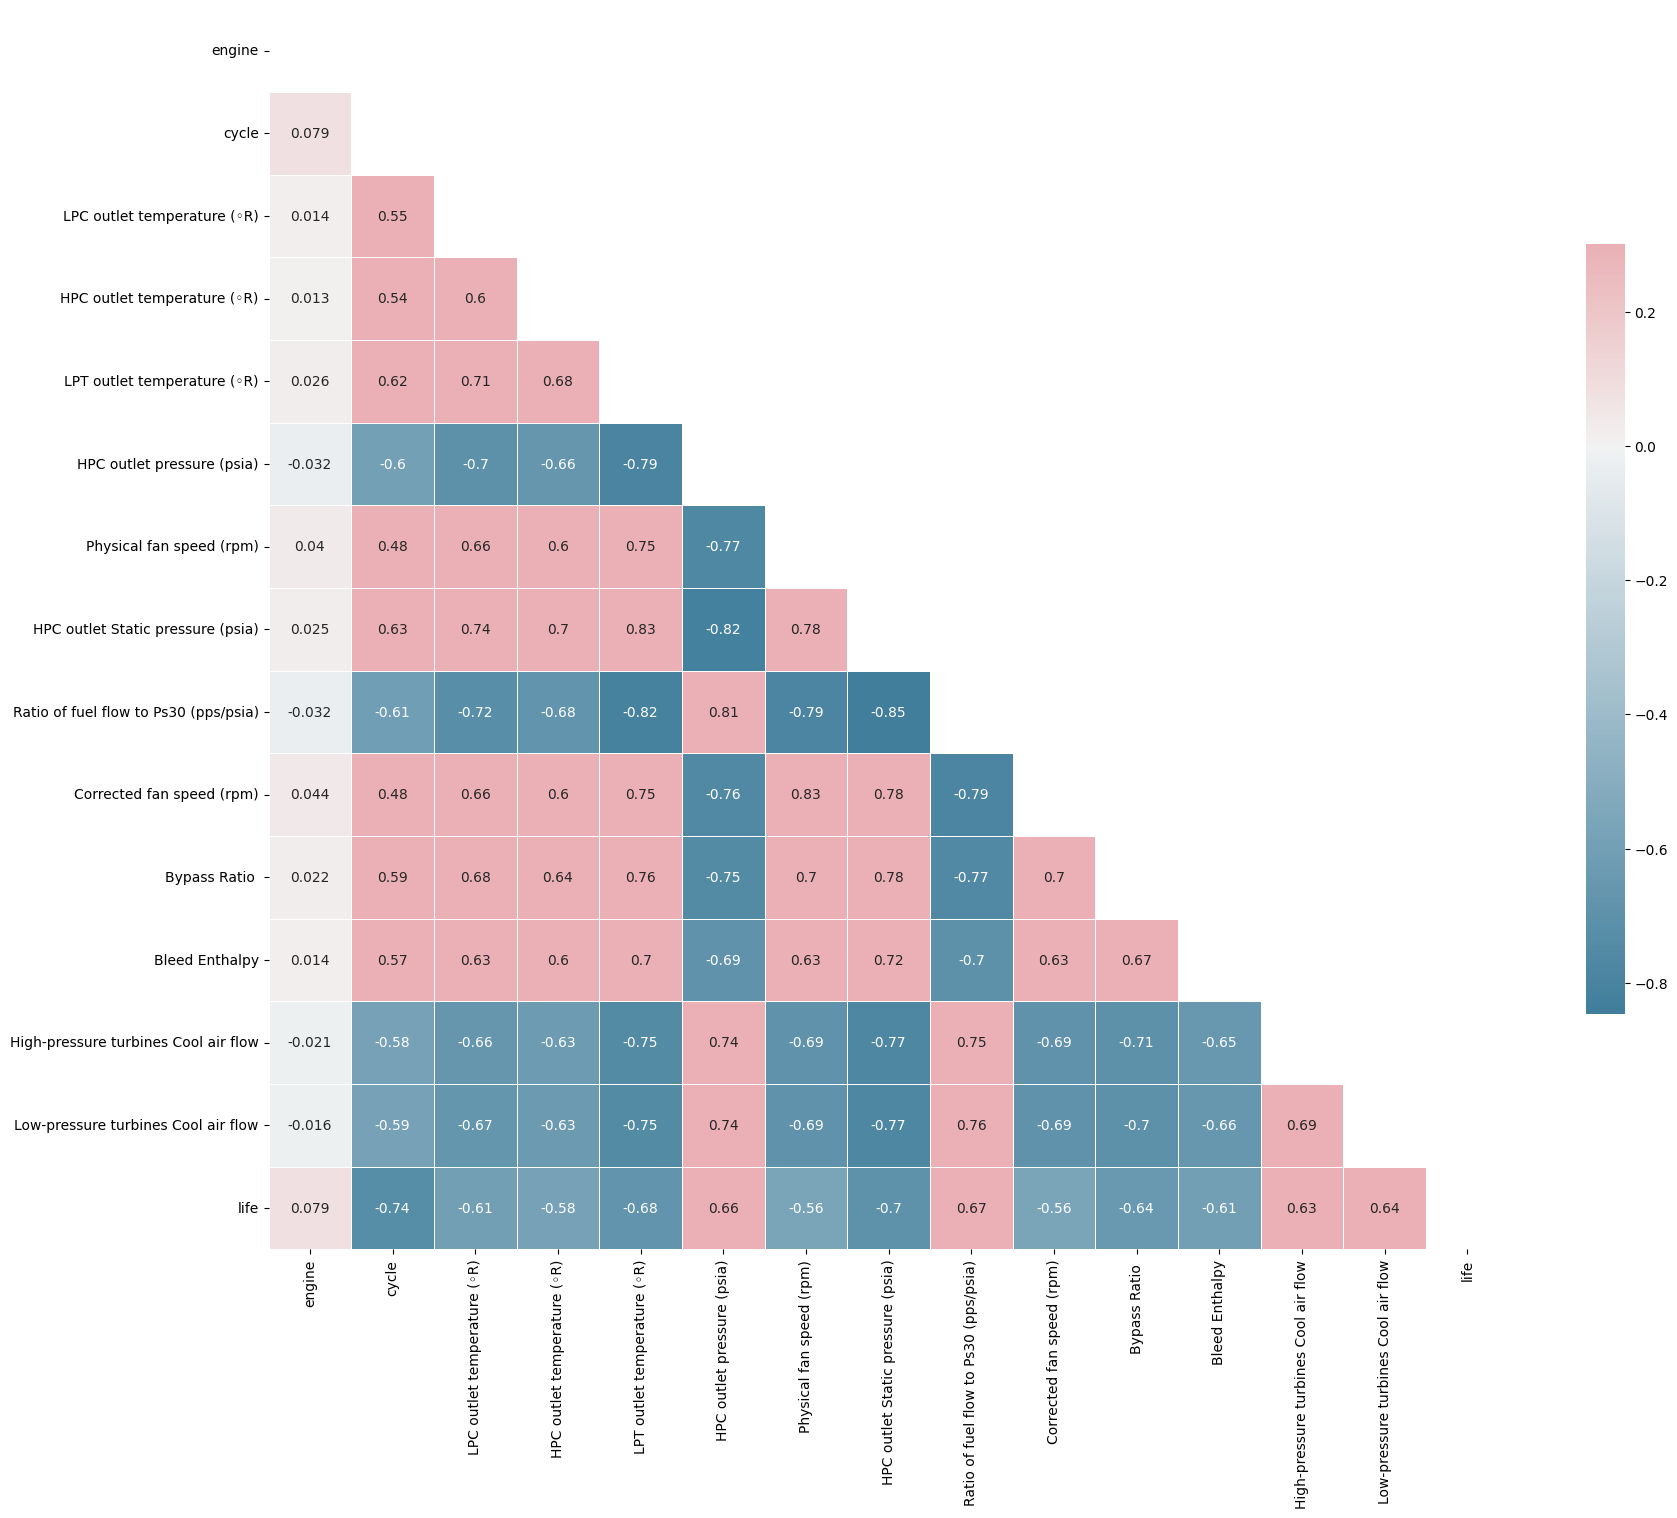
\includegraphics[width=0.8\textwidth]{images/correlation_matrix.png}
    \caption{Correlation matrix.}
    \label{fig:correlation_matrix}
\end{figure}



\subsubsection{Data smoothing}
After analyzing noise in the data, we applied a smoothing technique using an exponentially weighted moving average. A comparison between smoothed and non-smoothed sensor data is shown in Figure \ref{fig:smooth-comp}.  This technique was chosen to balance the trade-off between noise reduction and data lag. By smoothing the data, we improved the quality of the sensor readings, making them more reliable for predictive modeling. We visualized the smoothed data alongside the original data, which clearly showed the reduction in noise and highlighted the underlying trends more effectively. This visualization reaffirmed the importance of smoothing in enhancing the dataset's quality. By combining these preprocessing steps we prepared the dataset for effective modeling, ensuring that the features were relevant, the noise was minimized, and the data was ready for subsequent machine learning tasks.

\begin{figure}[h]
    \centering
    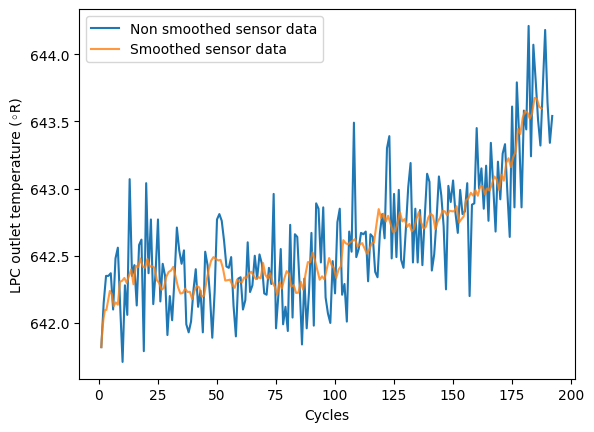
\includegraphics[width=0.7\textwidth]{images/smoothed_data_comaprison.png}
    \caption{Comparison of smoothed and non-smoothed sensor data.}
    \label{fig:smooth-comp}
\end{figure}

\subsubsection{Clipping Remaining Useful Life}

Our initial assumption for the Remaining Useful Life (RUL) in the training set is that it declines linearly to zero. However, sensor signals often exhibit a 'bend,' indicating the onset of degradation. Given the lack of information on initial wear and tear, this linear decline might not accurately represent the true RUL behavior.

To better reflect the observed data, we assume that the RUL remains constant initially and only begins to decline linearly after a certain point. This assumption has two main advantages:

\begin{itemize}
    \item Improved Correlation with Sensor Signals: By keeping the RUL constant initially, it aligns better with the stable mean of the sensor signals, providing a more realistic representation of the engine's life.
    \item Reduced Target Variable Spread: Lower peak RUL values result in a reduced spread of the target variable, making it easier to fit predictive models.
\end{itemize}

To implement this, we clip the RUL at a predefined value (e.g., 125 cycles), ensuring it remains constant up to this point before starting its linear decline. This clipping process is illustrated in Figure (figure \ref{fig:rul_cliping_comparison}), which shows how the RUL remains constant initially and then decreases linearly. This approach matches the patterns observed in the sensor data more closely, resulting in more accurate and reliable RUL predictions.

\begin{figure}[h]
    \centering
    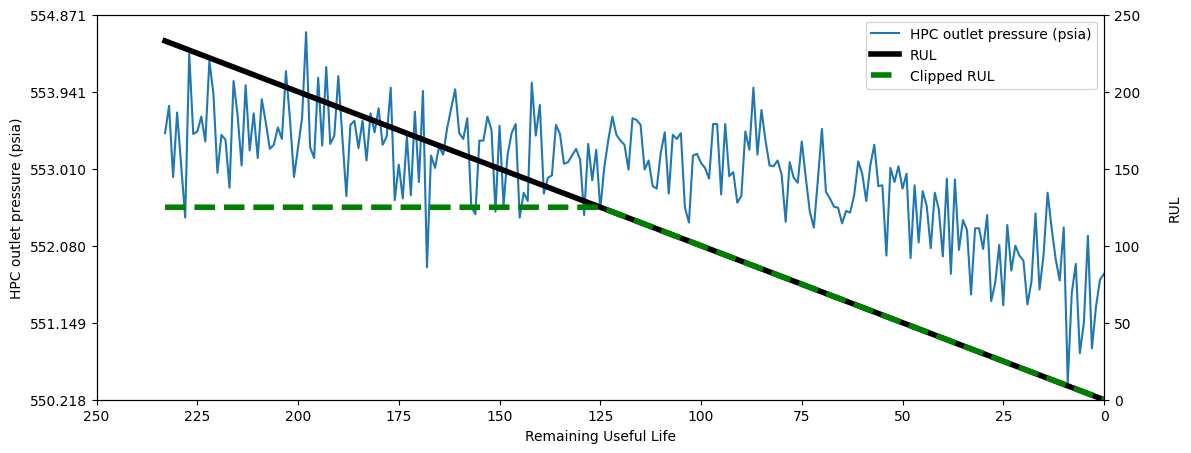
\includegraphics[width=0.9\textwidth]{images/rul_cliping_comparison.png}
    \caption{Clipping of RUL at value 125.}
    \label{fig:rul_cliping_comparison}
\end{figure}


\subsection{Machine Learning Methods}
For every model we splitted the dataset into a two smaller dataset, the train dataset and the test dataset, respectively the 70\% and 30 \% of the original dataset.

\subsubsection{Linear Regression}

Linear Regression is a simple yet powerful method for predicting a dependent variable ($y$) based on one or more independent variables ($x$) \cite{gujarati2019linear}. 
At its core, linear regression aims to find the best-fitting straight line through a set of data points. This line, known as the regression line, represents the predicted values of the dependent variable based on the values of the independent variables.

The relationship is modeled using a linear equation:

\begin{equation}
y = \beta_0 + \beta_1x_1 + \beta_2x_2 + \ldots + \beta_nx_n + \epsilon
\end{equation}

Here, $ y $ is the dependent variable, $ x $ is the independent variable, $ \beta_0 $ is the y-intercept, $ \beta_i $ are the coefficients, and $ \epsilon $ represents the error term, accounting for the variability in $ y $ that cannot be explained by the linear relationship with $ x $.
The coefficients ($\beta_i$) are estimated using the least squares method, which minimizes the sum of the squared differences between the observed and predicted values.

\textbf{Our implementation}

In our implementation, we created a pipeline that scaled the data with a MinMax Scaler before applying Linear Regression. The model was trained on the training data and evaluated using cross-validation (5 folds) on the four metrics described above. We visualized the predictions against the true values using a scatter plot (figure \ref{fig:linear_regression}), which helped us see how accurately the model predicted the data.

\begin{figure}[H]
    \centering
    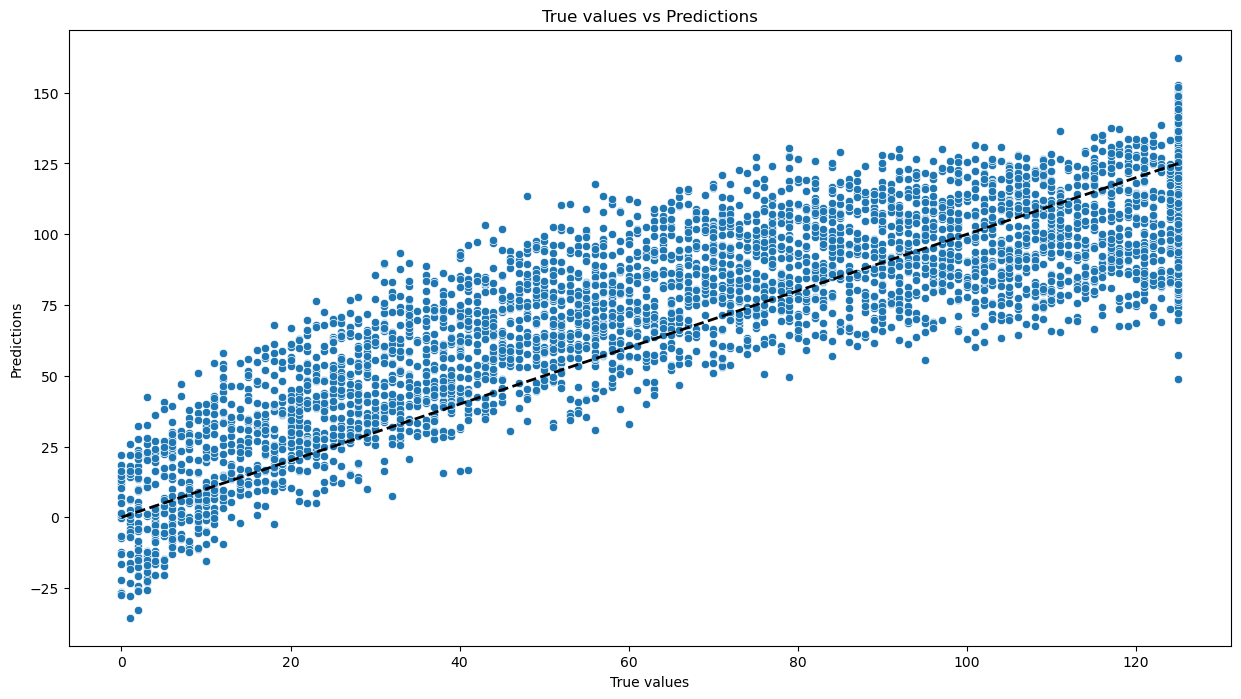
\includegraphics[width=0.8\textwidth]{images/linear_regression.png}
    \caption{Comparison of linear model predictions.}
    \label{fig:linear_regression}
\end{figure}

\subsubsection{Elastic Net}
 Elastic Net is a regularized regression method that linearly combines the L1 and L2 penalties of the Lasso and Ridge methods \cite{zou2005regularization}. It addresses the limitations of both methods, providing a balance between feature selection and coefficient shrinkage. 
 Elastic Net adds two types of regularization terms to the linear regression equation:
\begin{equation}
y = \beta_0 + \sum_{i=1}^{p} \beta_i x_i + \lambda_1 \sum_{i=1}^{p} |\beta_i| + \lambda_2 \sum_{i=1}^{p} \beta_i^2 + \epsilon
\end{equation}

Here, $ y $ is the dependent variable, $ x_i $ are the independent variables, $ \beta_i $ are the coefficients, $ \lambda_1 $ and $ \lambda_2 $ are the regularization parameters, and $ \epsilon $ is the error term. The regularization parameters are $ \lambda_1 $ and $ \lambda_2 $. $ \lambda_1 $ corresponds to the L1 norm (Lasso), promoting sparsity by encouraging some coefficients to be exactly zero. $ \lambda_2 $ corresponds to the L2 norm (Ridge), promoting smoothness by shrinking the coefficients towards zero, which helps handle multicollinearity and improve generalization\cite{zou2005regularization}\cite{friedman2010regularization}.
The optimization problem of Elastic Net regression involves finding the coefficients ($\beta$) that minimize both the residual sum of squares and regularization terms:

\begin{equation}
    \min_{\beta_0, \beta}  \frac{1}{2n} \sum_{i=1}^{n} (y_i - \beta_0 - \sum_{j=1}^{p} \beta_j x_{ij})^2 + \lambda_1 \sum_{j=1}^{p} |\beta_j| + \lambda_2 \sum_{j=1}^{p} \beta_j^2
\end{equation}

In this equation, $ n $ represents the number of observations, $ y_i $ is the dependent variable for observation $ i $, and $ x_{ij} $ is the value of the $ j $-th independent variable for observation $ i $. The intercept is $ \beta_0 $, and $ \beta_j $ are the coefficients.

\textbf{Our implementation}

In our practical implementation of the Elastic Net model, we combined L1 and L2 regularization to balance feature selection and coefficient shrinkage. We set up a pipeline with a StandardScaler and the Elastic Net model. Then we defined a grid of hyperparameters for Elastic Net and used GridSearchCV to find the best parameters. We visualized the evolution of the mean test scores against the hyperparameters to understand their impact (figure \ref{fig:elastic_net}). We got a result of 
\begin{verbatim}
    {'elasticnet__alpha': 0.0031622776601683794, 
    'elasticnet__l1_ratio': 0.001}
\end{verbatim}

\begin{figure}[H]
    \centering
    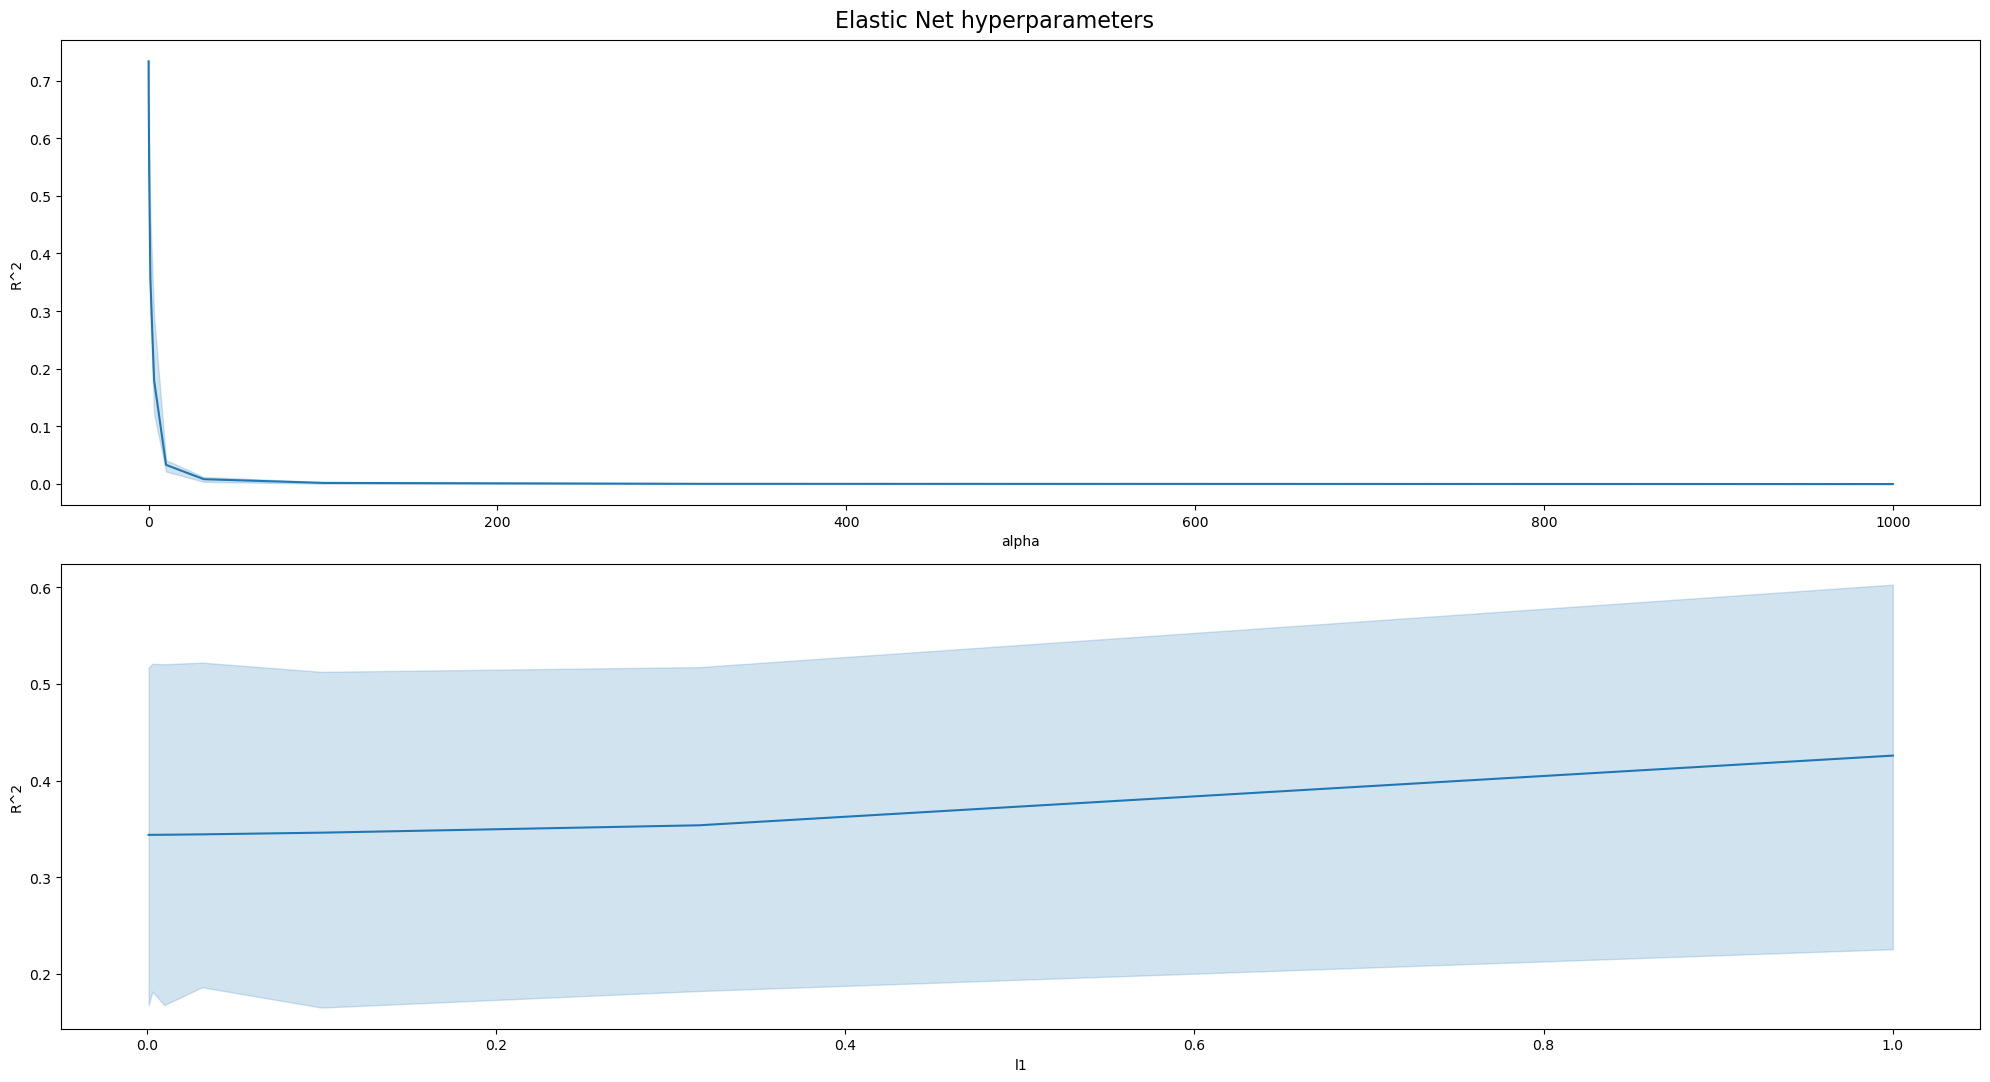
\includegraphics[width=1\textwidth]{images/elastic_net.png}
    \caption{Comparison of elastic net parameters.}
    \label{fig:elastic_net}
\end{figure}

We used a cross validation (5 folds) to get the scores of the best model. In the end we visualized the predictions against the true values using a scatter plot (figure \ref{fig:elastic_net_true_vs_fals}), as we did for the linear regression.

\begin{figure}[H]
    \centering
    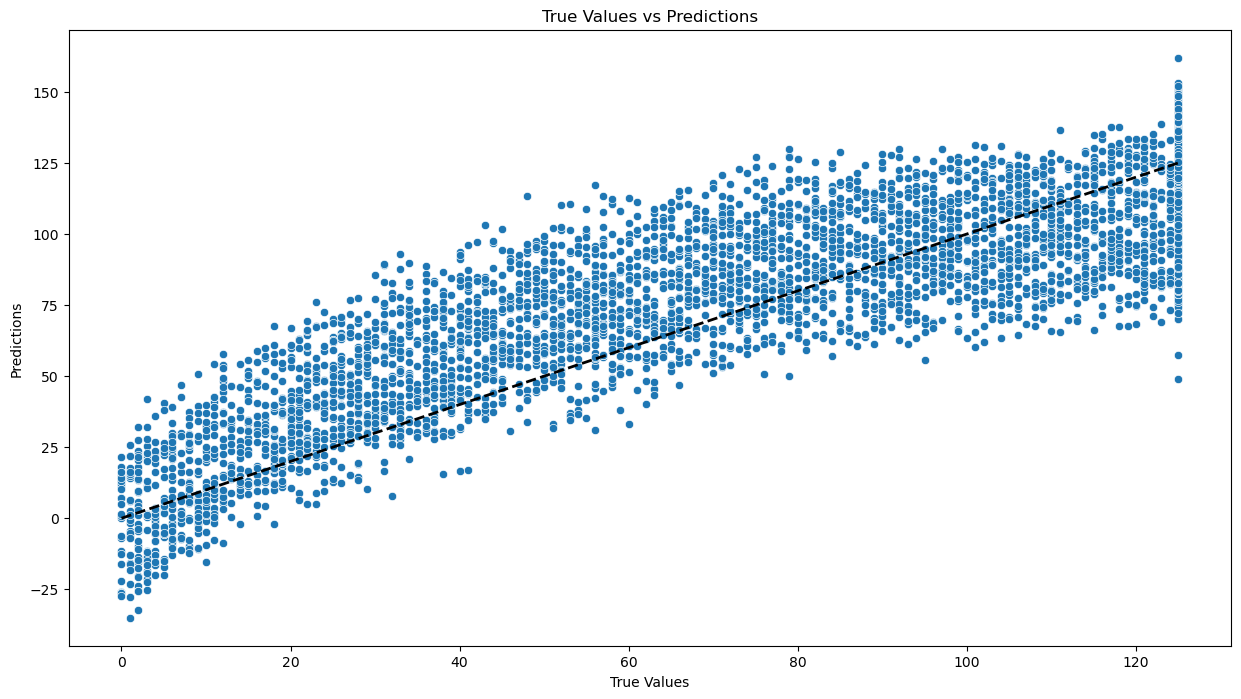
\includegraphics[width=0.8\textwidth]{images/elastic_net_true_vs_false.png}
    \caption{Comparison elastic net predictions.}
    \label{fig:elastic_net_true_vs_fals}
\end{figure}

\subsubsection{Regression Trees}
Regression trees are a type of decision tree specifically used for predicting continuous numerical outcomes. Regression Trees is a decision tree method used for predicting continuous values. Regression tree model is a non-parametric supervised learning method that recursively partitions the data space and fits a simple model (e.g., mean or median) within each partition, creating a tree-like model of decisions \cite{breiman1984classification}.

The Regression Tree algorithm involves the following steps:

\begin{enumerate}
    \item Start with the entire dataset as the root.
    \item At each node, split the dataset into two subsets based on the value of one of the independent variables. The split is chosen to minimize the mean squared error (MSE) within the resulting subsets.
    \item Repeat the splitting process recursively for each subset until a stopping criterion is met (e.g., minimum number of samples per leaf or maximum tree depth).
    \item Assign the mean value of the target variable within each terminal node (leaf) as the prediction for that region.
\end{enumerate}

\textbf{Our implementation}

In our practical implementation of Regression Trees, we aimed to predict continuous values by recursively partitioning the data and fitting simple models within each partition. We set up a pipeline with a MinMaxScaler and a Decision Tree Regressor. We defined a grid of hyperparameters for the regression tree and used GridSearchCV to find the best parameters and visualized the evolution of mean test scores against various hyperparameters (figure \ref{fig:regression_tree}) to understand their impact. 

For the best hyperparameters we got a result of 
\begin{verbatim}
    {'regressor_tree__max_depth': 10, 
    'regressor_tree__max_features': 0.6,
    'regressor_tree__min_samples_leaf': 20, 
    'regressor_tree__min_samples_split': 2}
\end{verbatim}

Then, using a cross-validate (10 folds) on the four metrics described above, we calculated the scores on both train and test datasets.

\begin{figure}[H]
    \centering
    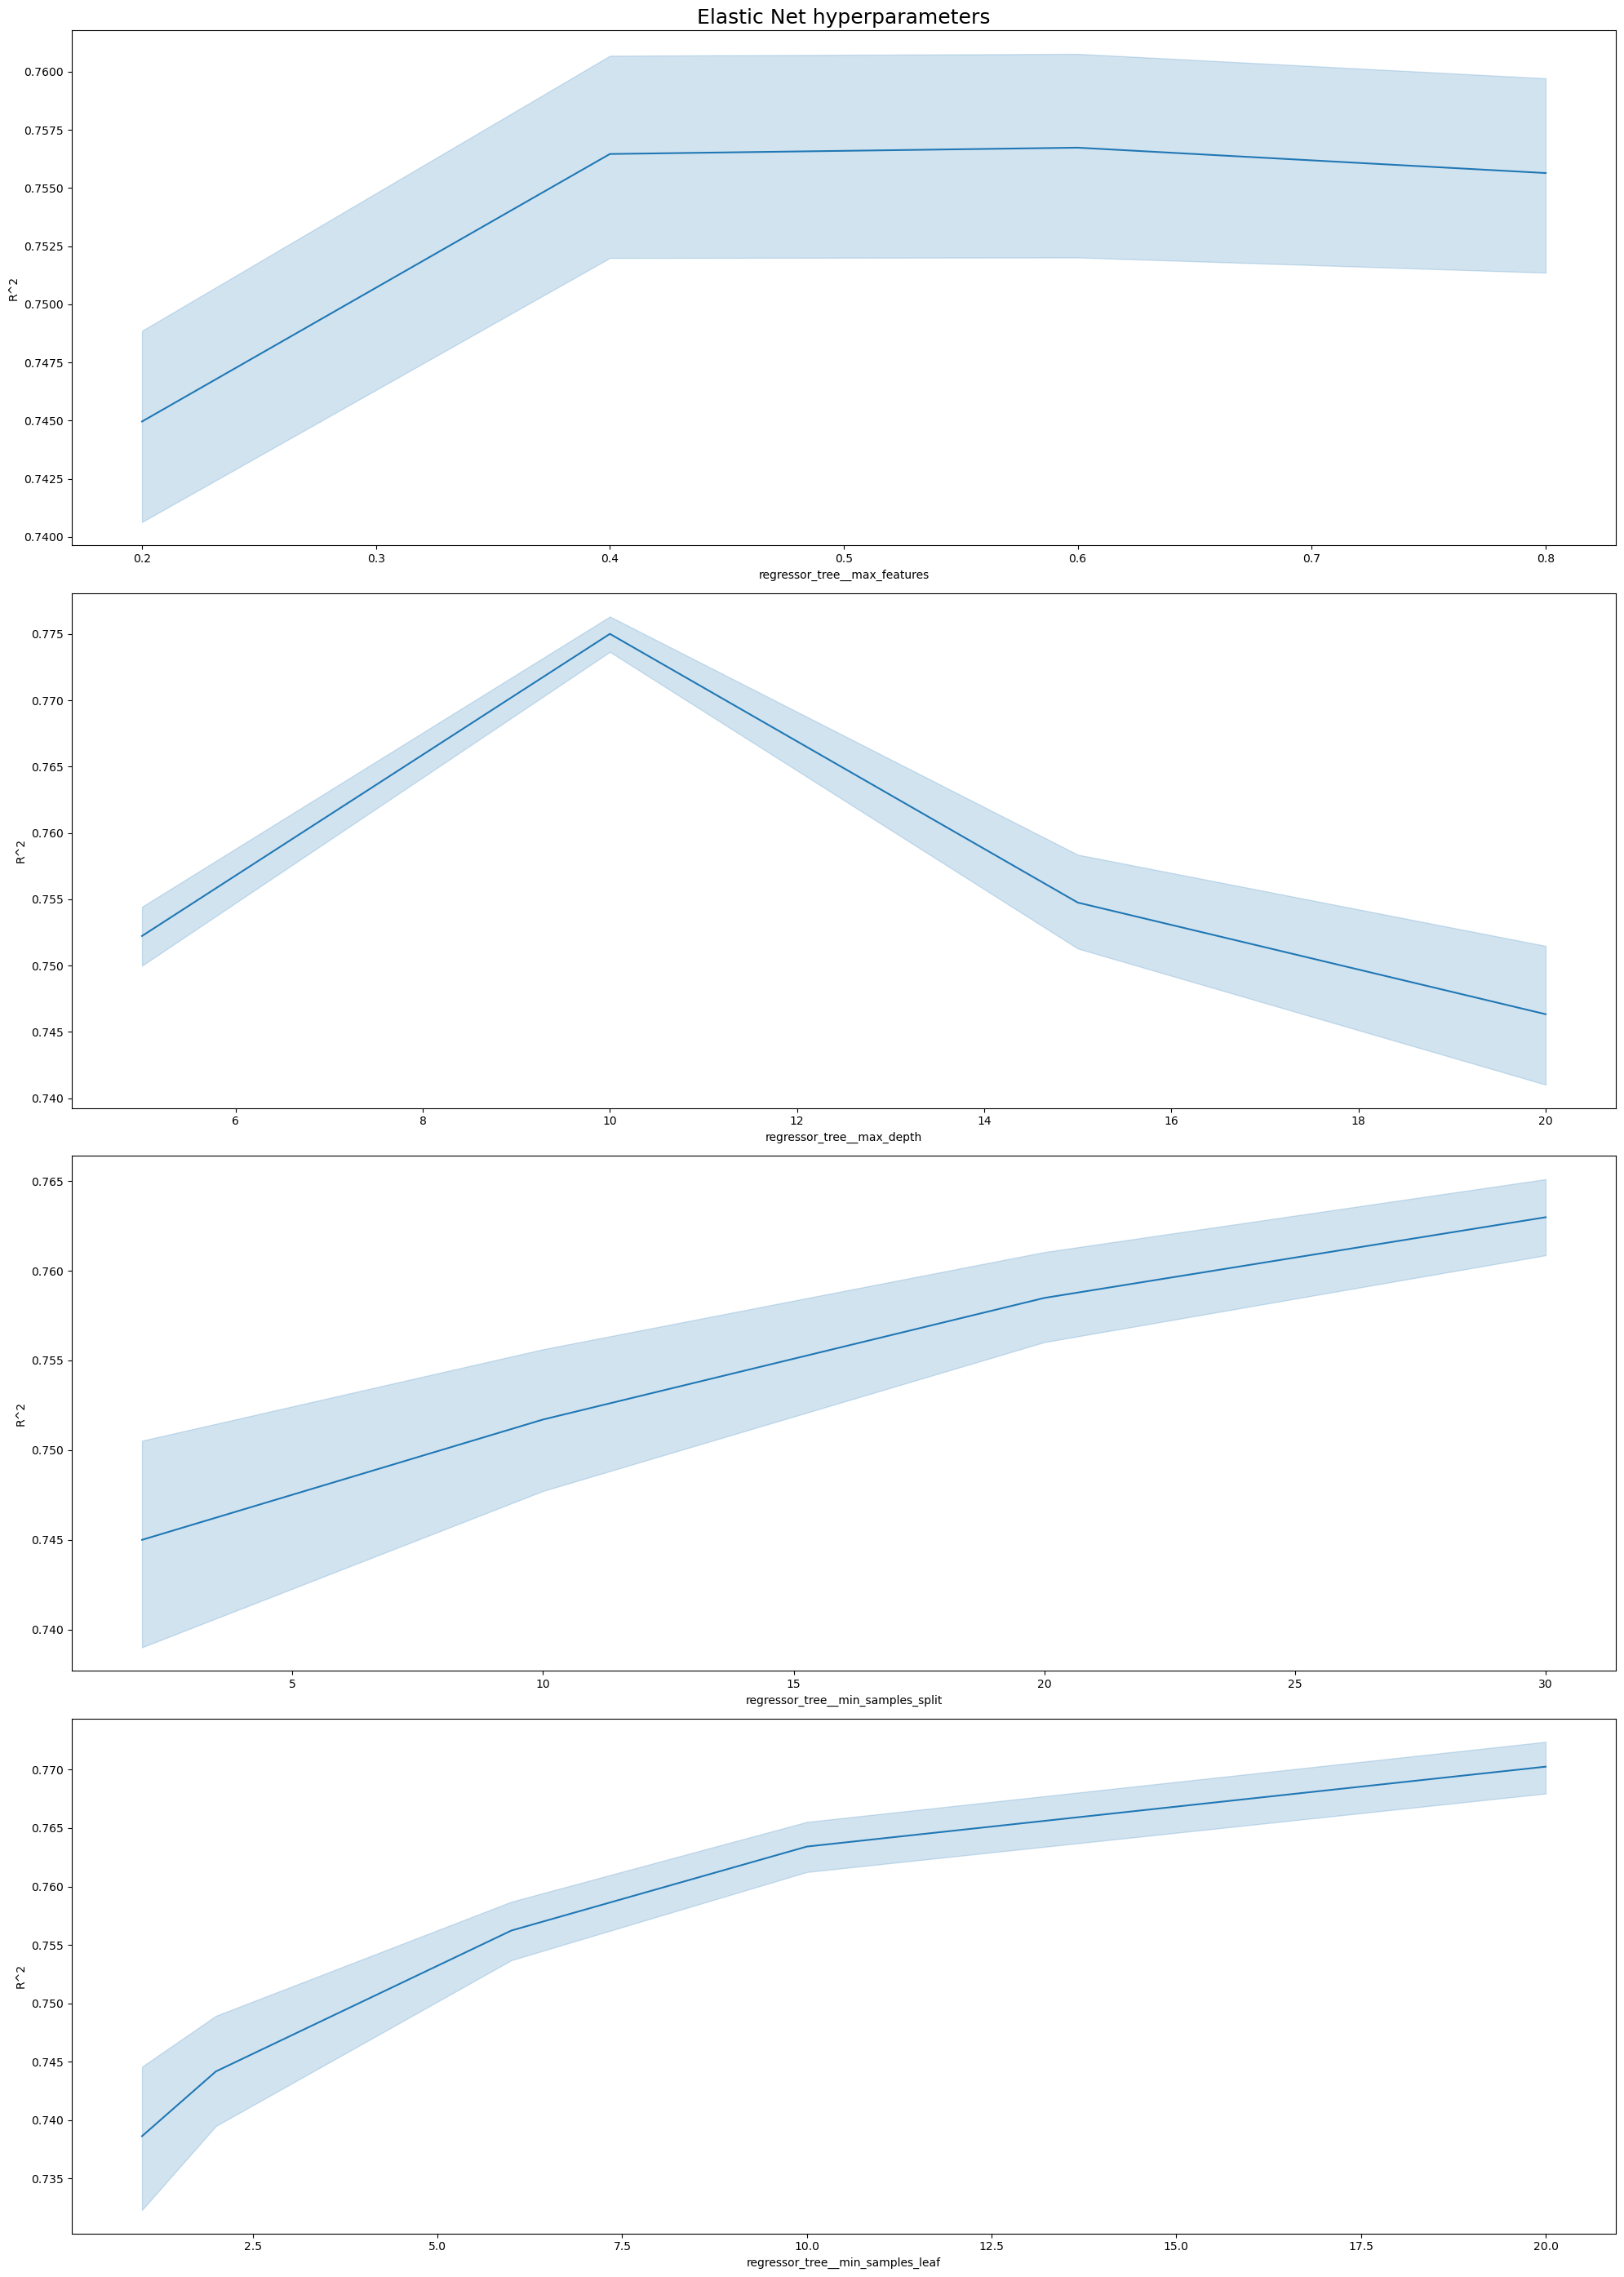
\includegraphics[width=0.8\textwidth]{images/regression_tree.png}
    \caption{Comparison of regression tree parameters.}
    \label{fig:regression_tree}
\end{figure}


\subsubsection{Support Vector Machines (SVM) regression}

Support Vector Machines (SVM) is a classification and regression algorithm that finds the hyperplane maximizing the margin between different classes \cite{Awad2015}. 
Support Vector Regression (SVR) is a supervised learning algorithm that is the regressional counterpart of Support Vector Machines (SVM) used for classification problems. While SVM aims to find a hyperplane that separates classes with the maximum margin, SVR aims to find a hyperplane that fits as many data points as possible within a specified margin. This hyperplane is determined by a subset of training samples known as support vectors.

The optimization problem for a linear SVM is:

\begin{equation}
\min \frac{1}{2} ||w||^2 \text{ s.t } y_i (w \cdot x_i + b) \ge 1, \text{ for all } i
\end{equation}

Here $w$ is the weight vector, $b$ is the bias term, $y_i$ is the class label and $x_i$ is the feature vector

Similar to SVM, SVR can utilize kernel functions to transform the input data into a higher-dimensional feature space \cite{dataflair_svm_kernel}. Kernels allow SVR to handle non-linear relationships between input and output variables by implicitly mapping them to a higher-dimensional space where they may become linearly separable. In our implementation we used both linear and RBF kernels to compare their performance.

\textbf{Our implementation}

We set up a pipeline with a StandardScaler and an SVM regressor with a linear kernel.
Using GridSearchCV, we tuned the hyperparameters to identify the best model, and we visualized the impact of the hyperparameters (figure \ref{fig:linear_SVM_regressor}).

For the best model we got a result of 
\begin{verbatim}
    {'svm__C': 0.3981071705534973,
    'svm__gamma': 0.01}
\end{verbatim}

We evaluated the model's performance on the training and test datasets using cross-validation (10 folds), 

\begin{figure}[H]
    \centering
    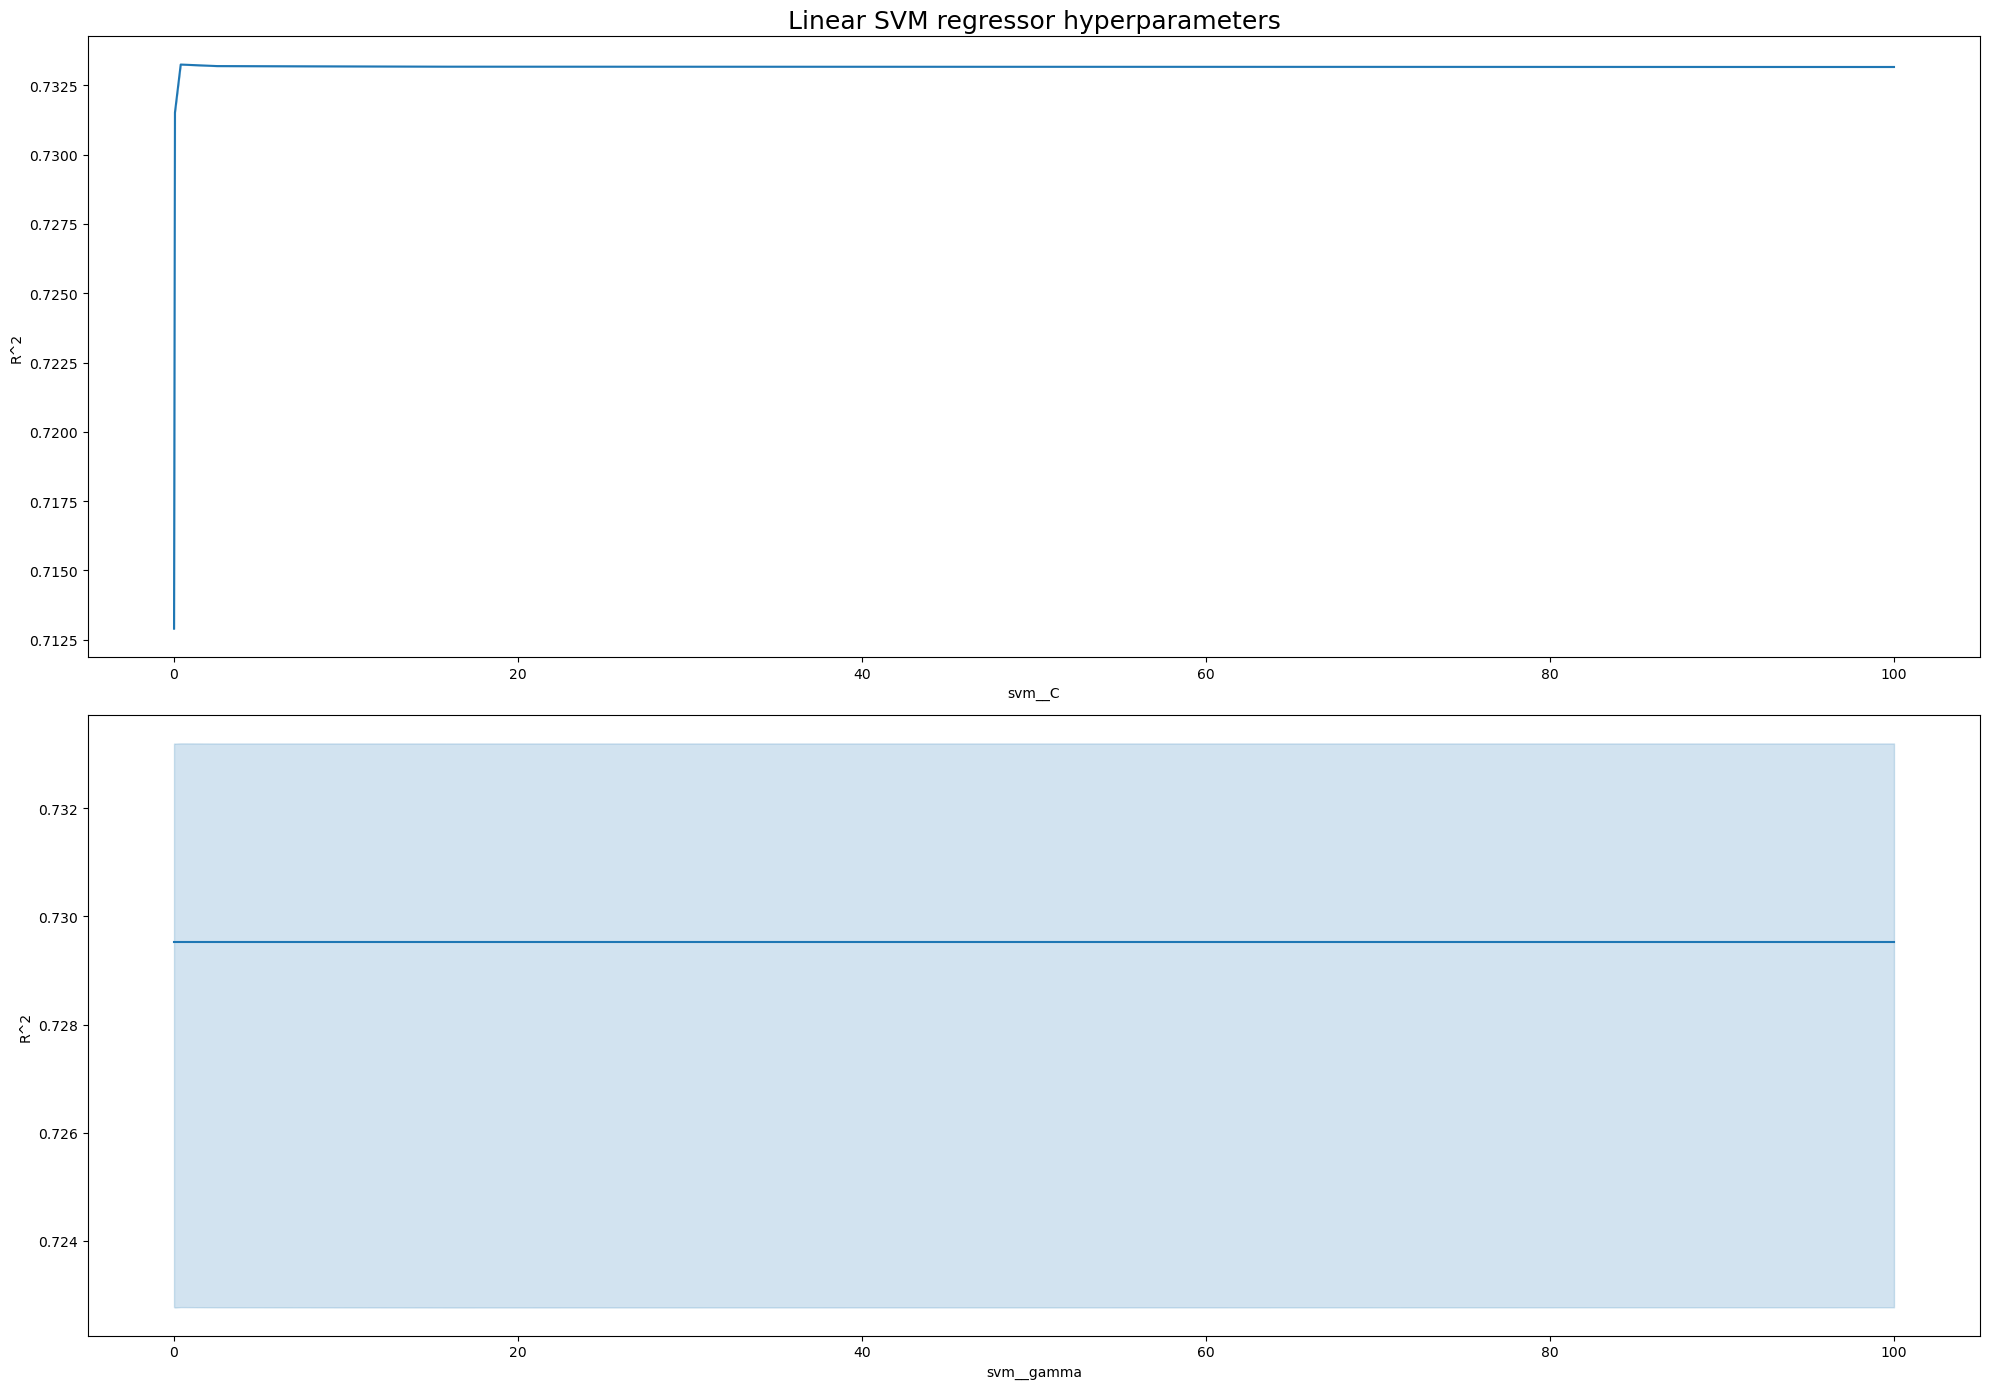
\includegraphics[width=0.7\textwidth]{images/linear_SVM_regressor.png}
    \caption{Comparison of linear SVM regressor parameters.}
    \label{fig:linear_SVM_regressor}
\end{figure}

Similarly, we created a pipeline for the SVM regressor with an RBF kernel. After tuning the hyperparameters with GridSearchCV, we found the best model. We got a result of \begin{verbatim}
    {'svm__C': 100.0, 
    'svm__gamma': 2.5118864315095824}
\end{verbatim}
As for the linear kernel SVR we visualized the parameter evolution to understand their effect on the model's performance (figure \ref{fig:rbf_SVM_regressor}).

Then, using a cross validatiom (10 folds) we assessed the best model's performance on both the training and test datasets.

\begin{figure}[H]
    \centering
    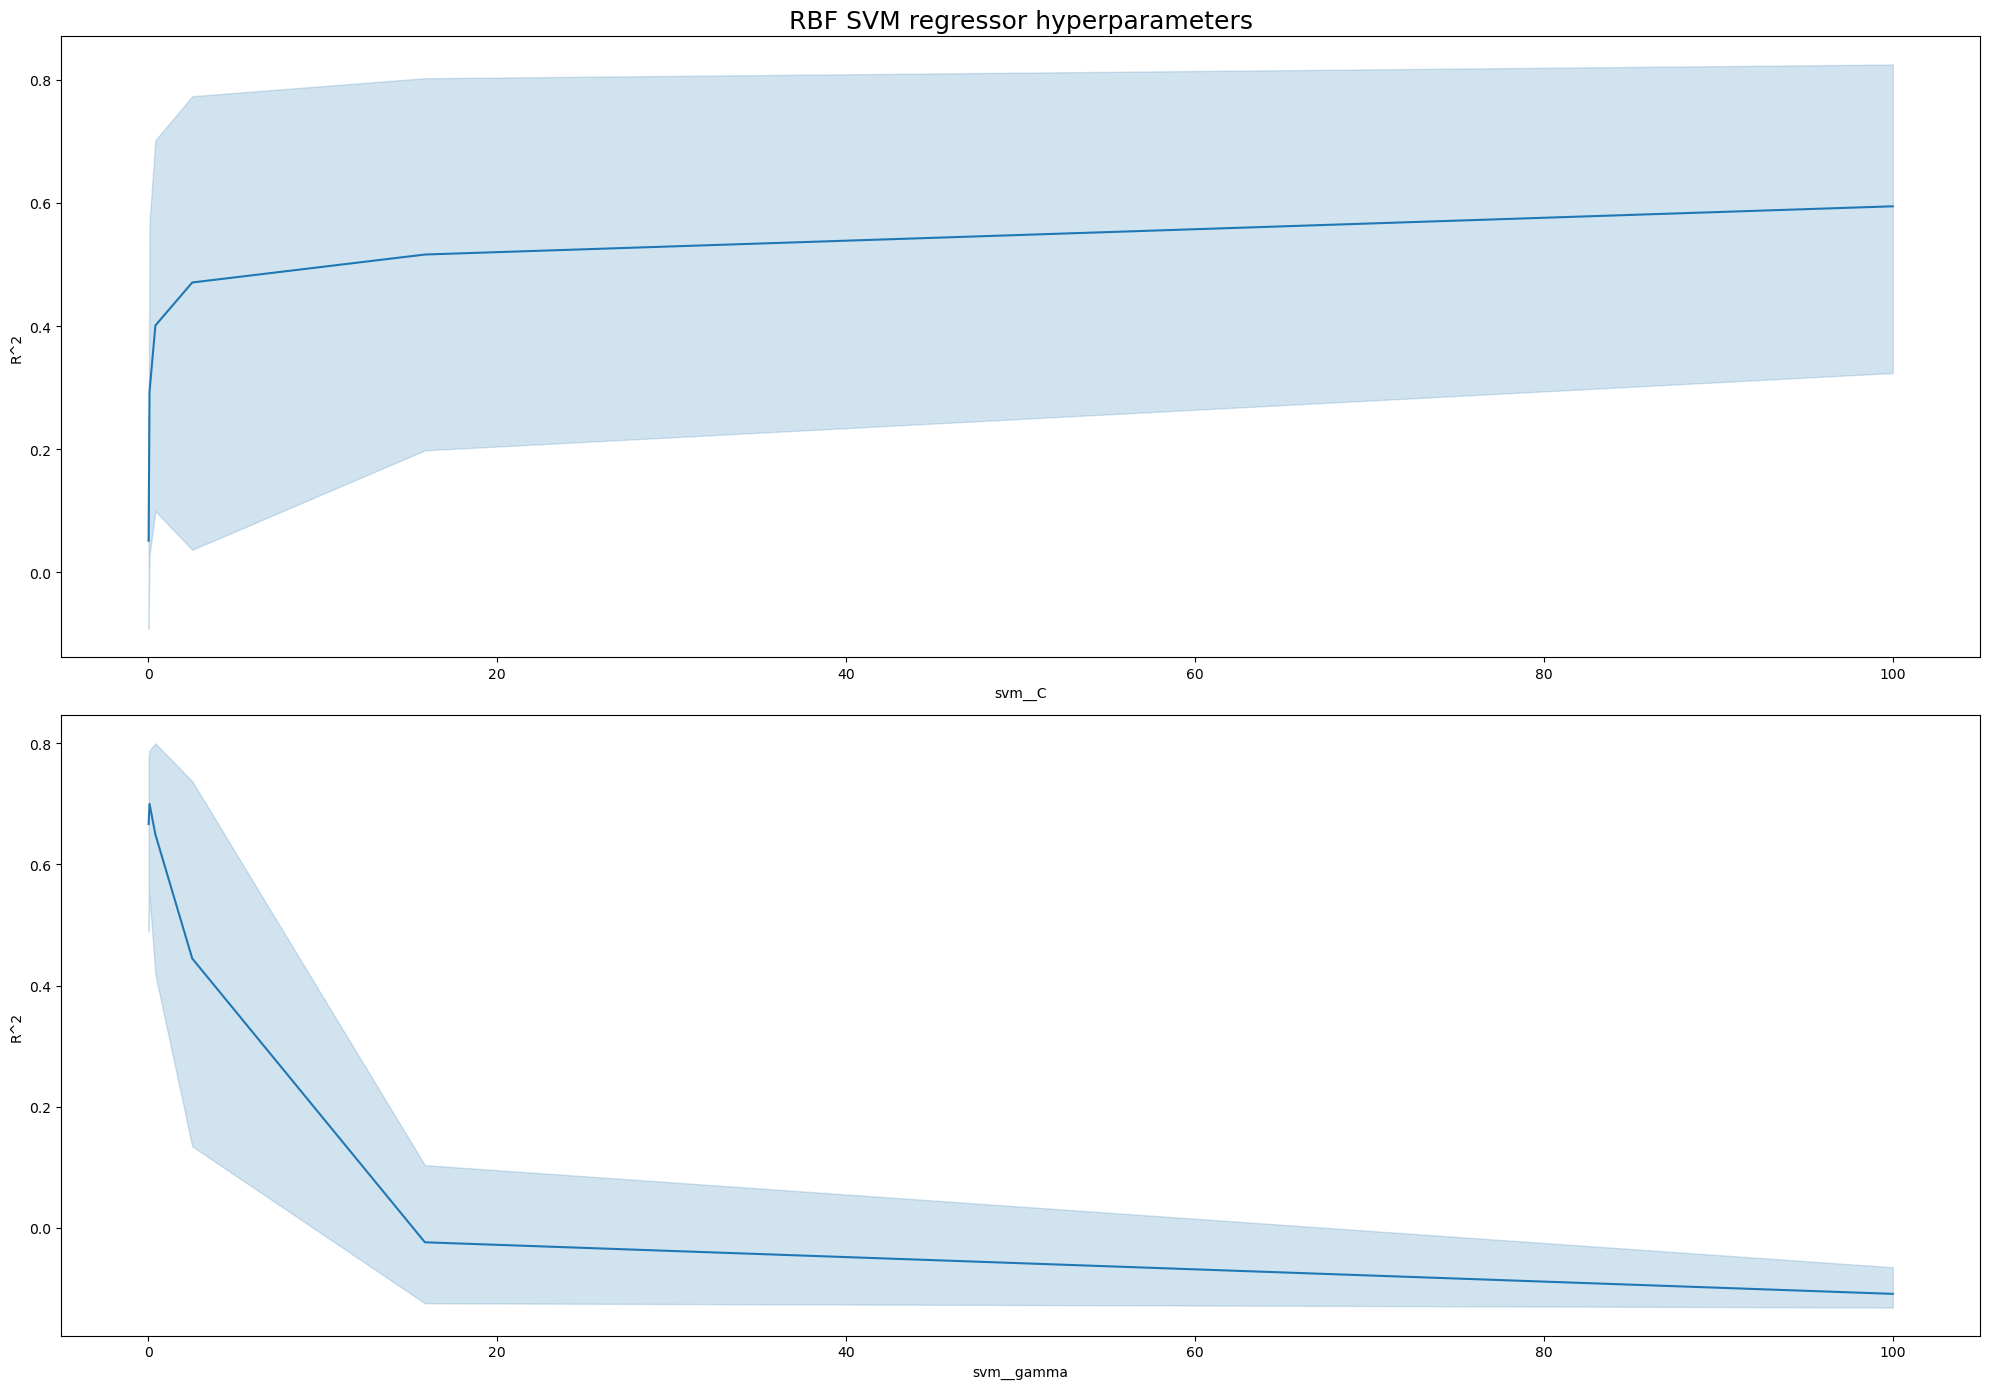
\includegraphics[width=0.7\textwidth]{images/rbf_SVM_regressor.png}
    \caption{Comparison of RBF SVM regressor parameters.}
    \label{fig:rbf_SVM_regressor}
\end{figure}


\subsubsection{Random Forests}

Random Forests is an ensemble learning technique that constructs multiple decision trees during training and aggregates their outputs to improve predictive accuracy. Each tree in the forest is built from a random subset of the training data, and at each split in the tree, a random subset of features is considered \cite{Breiman2001}.

More in detail Regression trees within a Random Forest are built using bootstrap samples of the training data. At each node, a random subset of features is selected, and the best split is chosen to minimize the mean squared error. This randomness helps create diverse trees, which collectively provide a more robust and generalized model. 
The predictions of all trees are averaged to produce the final output, which reduces variance and improves robustness compared to a single tree \cite{liaw2002classification}. This ensemble approach mitigates the risk of overfitting. 

The theoretical strength of Random Forest regression comes from its ability to manage the bias-variance tradeoff effectively, leading to lower generalization error. The combination of bootstrap sampling, feature randomness, and aggregation enhances model stability and accuracy \cite{Biau2016}. 

Random Forests provide also a natural way to estimate feature importance by measuring the impact of each feature on the prediction accuracy \cite{Breiman2001}.
The main steps of the Random Forest algorithm are:
\begin{enumerate}
    \item Draw B bootstrap samples from the training data.
    \item For each bootstrap sample, grow an unpruned decision tree:
    \begin{enumerate}
        \item At each node, select a random subset of m predictors.
        \item Split the node using the best predictor among the subset.
    \end{enumerate}
    \item Aggregate the predictions of the B trees to make the final prediction.
\end{enumerate}

\textbf{Our implementation}

In our implementation of Random Forests, we started by defining a pipeline with a StandardScaler and a RandomForestRegressor, enabling the score to evaluate the model using out-of-bag samples. 

We created a grid of hyperparameters to identify the optimal combination of hyperparameters that maximizes the model's performance. We performed the tuning using GridSearchCV and we got as a result: 
\begin{verbatim}
    {'random_forest__max_depth': 20, 
    'random_forest__max_features': 10,
    'random_forest__n_estimators': 300}
\end{verbatim}

We visualized the performance trends by plotting the evolution of mean test scores as hyperparameters vary (figure \ref{fig:random_forest}). Using cross validation (10 folds), we evaluated the performance of the tuned Random Forest Regressor on both the training and test datasets on the performance metrics described above.

We displayed also the out-of-bag (OOB) score of the Random Forest Regressor. to estimate the performance of the model without the need for a separate validation dataset. This metric provides an estimate of the model's predictive accuracy using unseen data. We got as a result:
\begin{verbatim}
    OOB Score: 0.84895
\end{verbatim}


To gain further insights, we analyzed and plotted the feature importance, highlighting which features contributed most to the model’s predictions (figure \ref{fig:random_forest_features}). 

\begin{figure}[H]
    \centering
    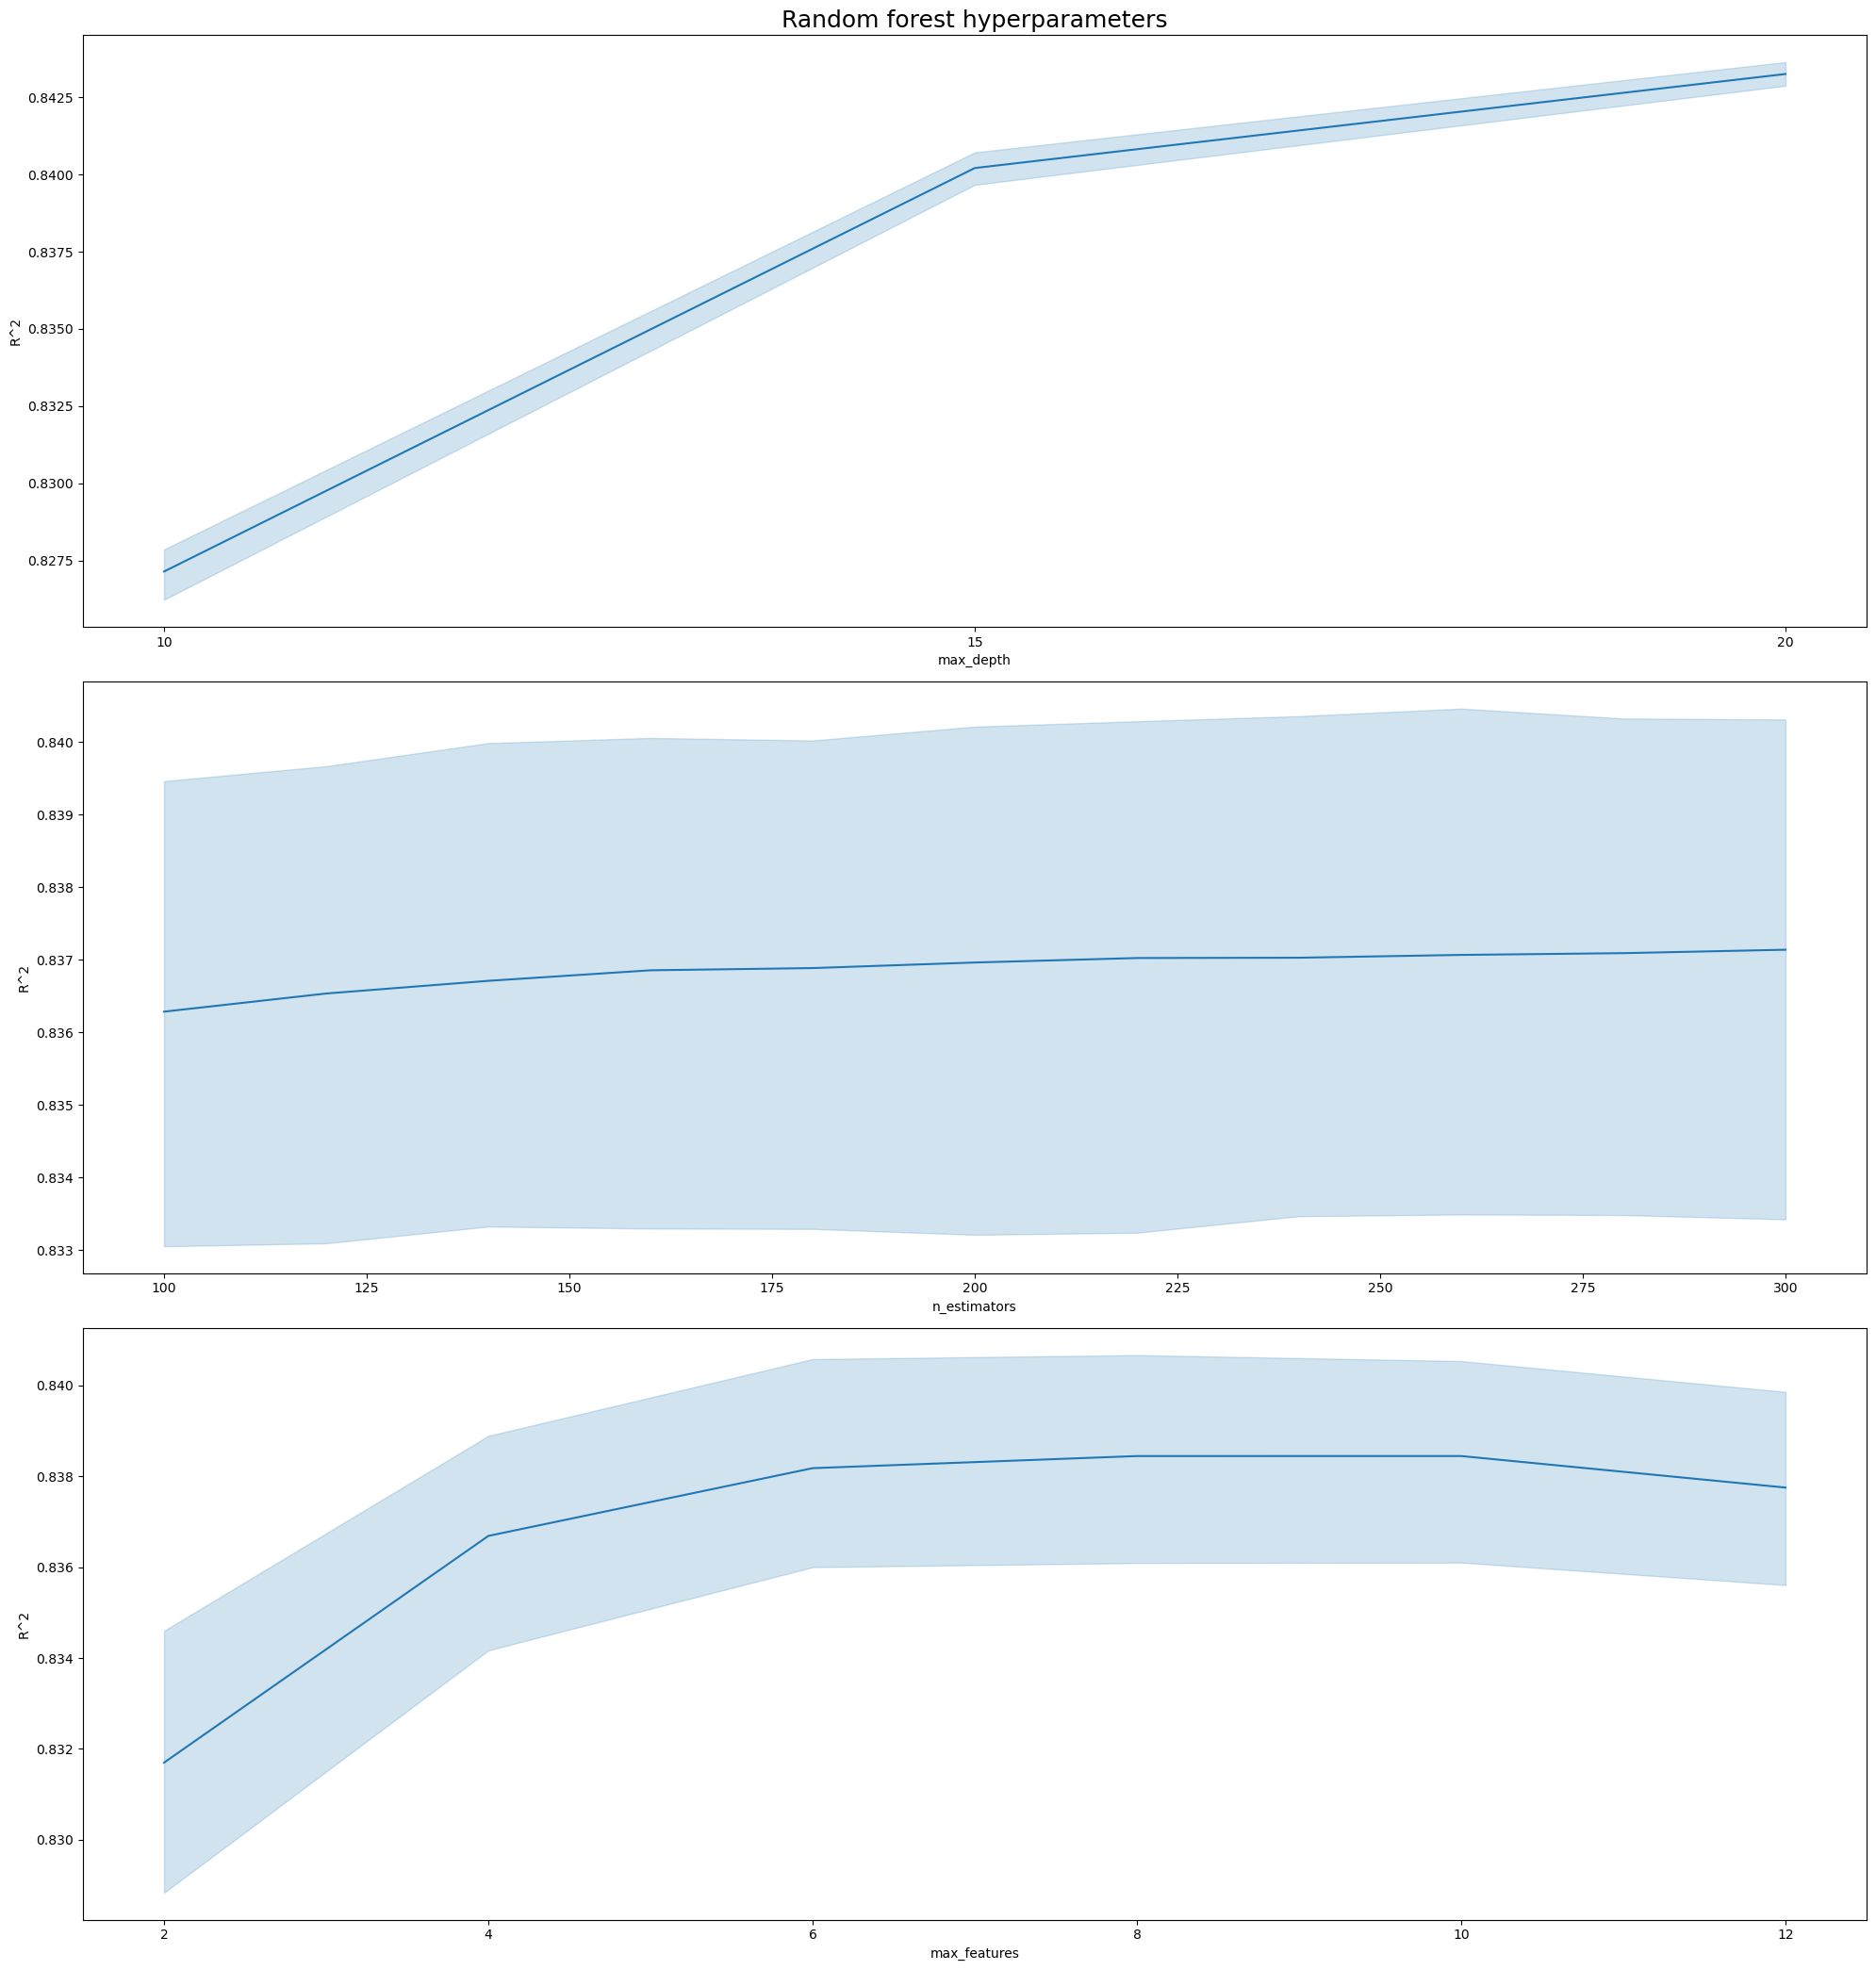
\includegraphics[width=0.9\textwidth]{images/random_forest.png}
    \caption{Comparison of random forest parameters.}
    \label{fig:random_forest}
\end{figure}

\begin{figure}[H]
    \centering
    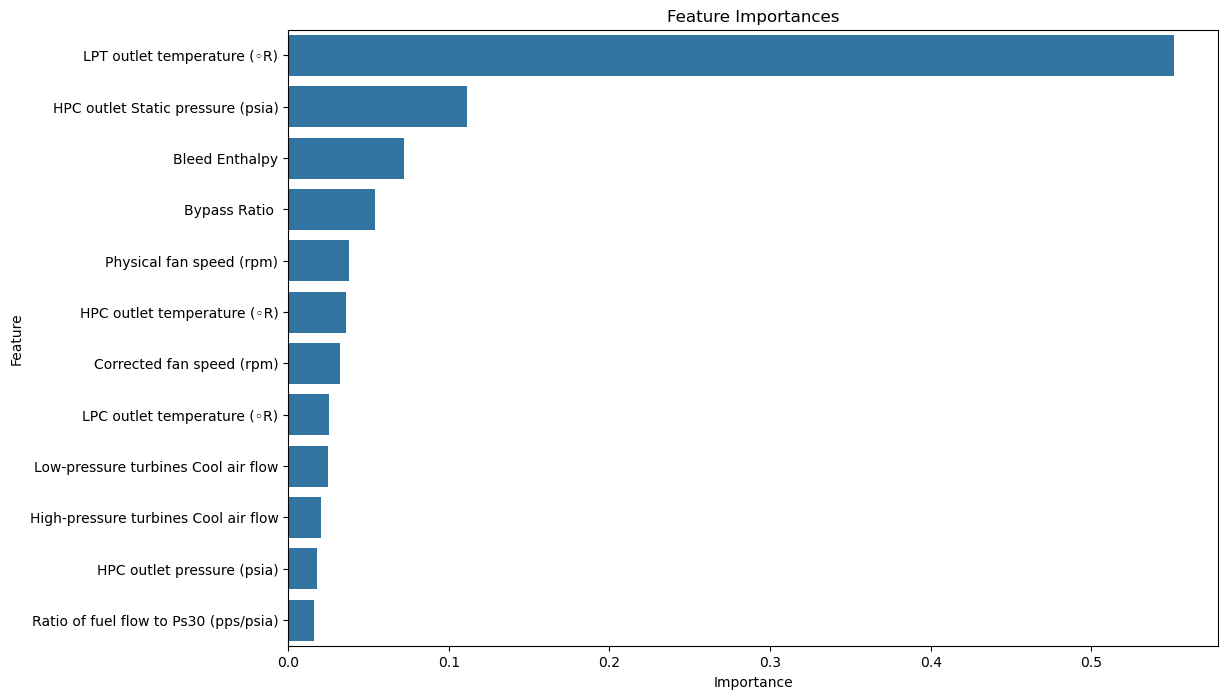
\includegraphics[width=0.8\textwidth]{images/random_forest_features.png}
    \caption{Analyzed feature importance for random forest model.}
    \label{fig:random_forest_features}
\end{figure}

\subsubsection{Neural Network}

A neural network is a computational model inspired by the human brain, consisting of interconnected nodes (neurons) that process data in layers to recognize patterns and make predictions. 

\textbf{Our implementation}

The best-performing model was composed by a network with two hidden layers, composed respectively by 32 and 16 neurons, as shown in the following summary (figure \ref{fig:model_nn}):

\begin{figure}[H]
    \centering
    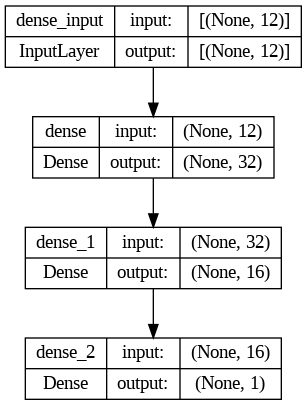
\includegraphics[width=0.3\textwidth]{images/model_nn.png}
    \caption{Neural network summary.}
    \label{fig:model_nn}
\end{figure}

The model has been trained with a batch size of 16 for 250 epochs. It reserves 10\% of the training data for validation and includes an early stopping callback that monitors the mean squared error. The training will stop if there is no improvement in the error for 20 consecutive epochs and will restore the model weights to the best observed during training. The following graphs shows the values of MSE (figure \ref{fig:MSE_nn}), RMSE (figure \ref{fig:RMSE_nn}), MAE (figure \ref{fig:MAE_nn}) and R² (figure \ref{fig:R2_nn}) of both training and validation splits during each training epoch:

\begin{figure}[H]
    \centering
    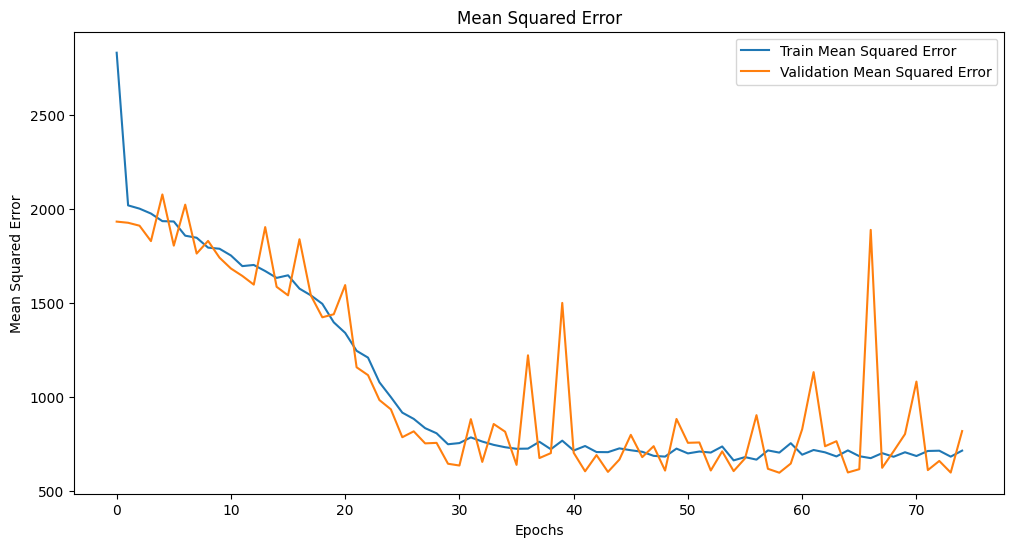
\includegraphics[width=0.6\textwidth]{images/MSE_nn.png}
    \caption{Neural Network Mean Square Error.}
    \label{fig:MSE_nn}
\end{figure}

\begin{figure}[H]
    \centering
    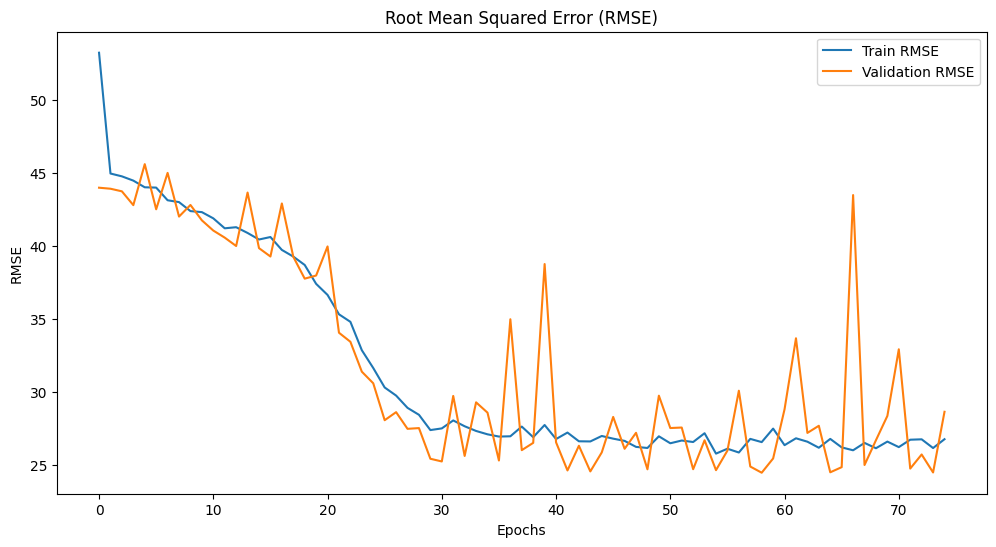
\includegraphics[width=0.6\textwidth]{images/RMSE_nn.png}
    \caption{Neural Network Root Mean Square Error.}
    \label{fig:RMSE_nn}
\end{figure}

\begin{figure}[H]
    \centering
    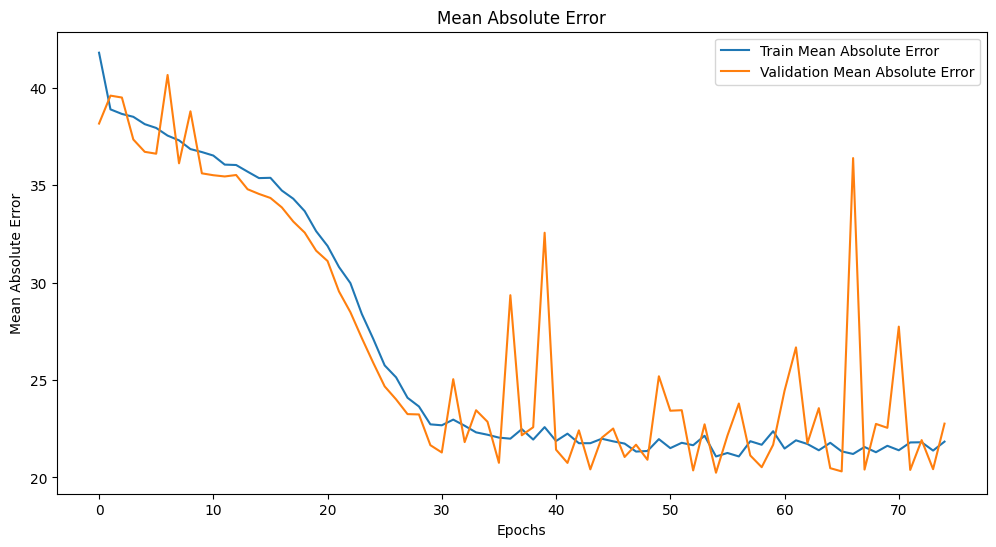
\includegraphics[width=0.6\textwidth]{images/MAE_nn.png}
    \caption{Neural Network Mean Absolute Error.}
    \label{fig:MAE_nn}
\end{figure}

\begin{figure}[H]
    \centering
    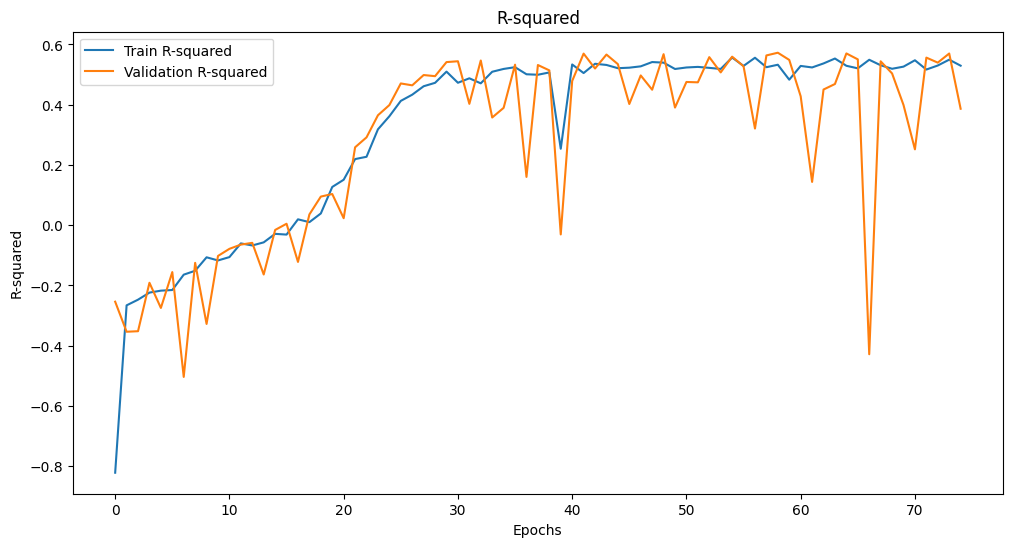
\includegraphics[width=0.6\textwidth]{images/R2_nn.png}
    \caption{Neural Network R².}
    \label{fig:R2_nn}
\end{figure}

\subsection{Software}
The models were developed using the Python libraries Pandas, NumPy, and scikit-learn (SKlearn) \cite{numpy}\cite{pandas}\cite{scikit-learn}. SKlearn was the primary contributor, offering a comprehensive array of tools essential for machine learning, including pre-processing utilities, various machine learning algorithms, and evaluation metrics. For data visualization and plotting, seaborn and matplotlib were utilized \cite{seaborn}\cite{matplotlib}.

\section{Results and Discussion}

Our project evaluated several machine learning models for predicting the remaining useful life (RUL) of turbofan engines, including Linear Regression, Elastic Net, Random Forests, Support Vector Machines (SVM), and Regression Trees. On the given dataset, we utilized data from sensors with preprocessing steps such as data cleaning, smoothing, and feature selection to enhance model performance. For better comparison on all tested models, we listed cross-validation methods for train set in table (table \ref{table:train_model_performance}) and (figure \ref{fig:train_model}). Detailed test results of our experiments are also evaluated in table (table \ref{table:test_model_performance}) and comparison chart (figure \ref{fig:test_model}).

\begin{table}[ht]
\centering
\begin{tabular}{|l|c|c|c|}
\hline
\textbf{Model} & $\mathbf{R^2}$ & \textbf{Mean Absolute Error} & \textbf{Root Mean Squared Error} \\ \hline
Neural network & 0.650 & 19.444 & 23.927 \\ \hline
SVM regression - linear kernel& 0.733 & 17.602 & 21.611 \\ \hline
Linear Regression & 0.734 & 17.569 & 21.579 \\ \hline
Elastic Net Models & 0.734 & 17.573 & 21.574 \\ \hline
Regression Tree & 0.782 & 13.796 & 19.526 \\ \hline
Random forest & 0.845 & 11.011 & 16.480 \\ \hline
SVM regression - rbf kernel & 0.869 & 10.275 & 15.114 \\ \hline
\end{tabular}
\caption{Comparison of Model Performance on train set.}
\label{table:train_model_performance}
\end{table}


\begin{table}[ht]
\centering
\begin{tabular}{|l|c|c|c|}
\hline
\textbf{Model} & $\mathbf{R^2}$ & \textbf{Mean Absolute Error} & \textbf{Root Mean Squared Error} \\ \hline
Neural network & 0.630 & 19.592 & 24.107 \\ \hline
SVM regression - linear kernel& 0.722 & 17.627 & 21.693 \\ \hline
Elastic Net & 0.723 & 17.626 & 21.678 \\ \hline
Linear Regression Models & 0.723 & 17.607 & 21.678 \\ \hline
Regression Tree & 0.757 & 14.267 & 20.292 \\ \hline
SVM regression - rbf kernel& 0.801 & 13.062 & 18.346 \\ \hline
Random forest & 0.814 & 12.904 & 17.742 \\ \hline
\end{tabular}
\caption{Comparison of Model Performance on Test Set}
\label{table:test_model_performance}
\end{table}


\begin{figure}[H]
    \centering
    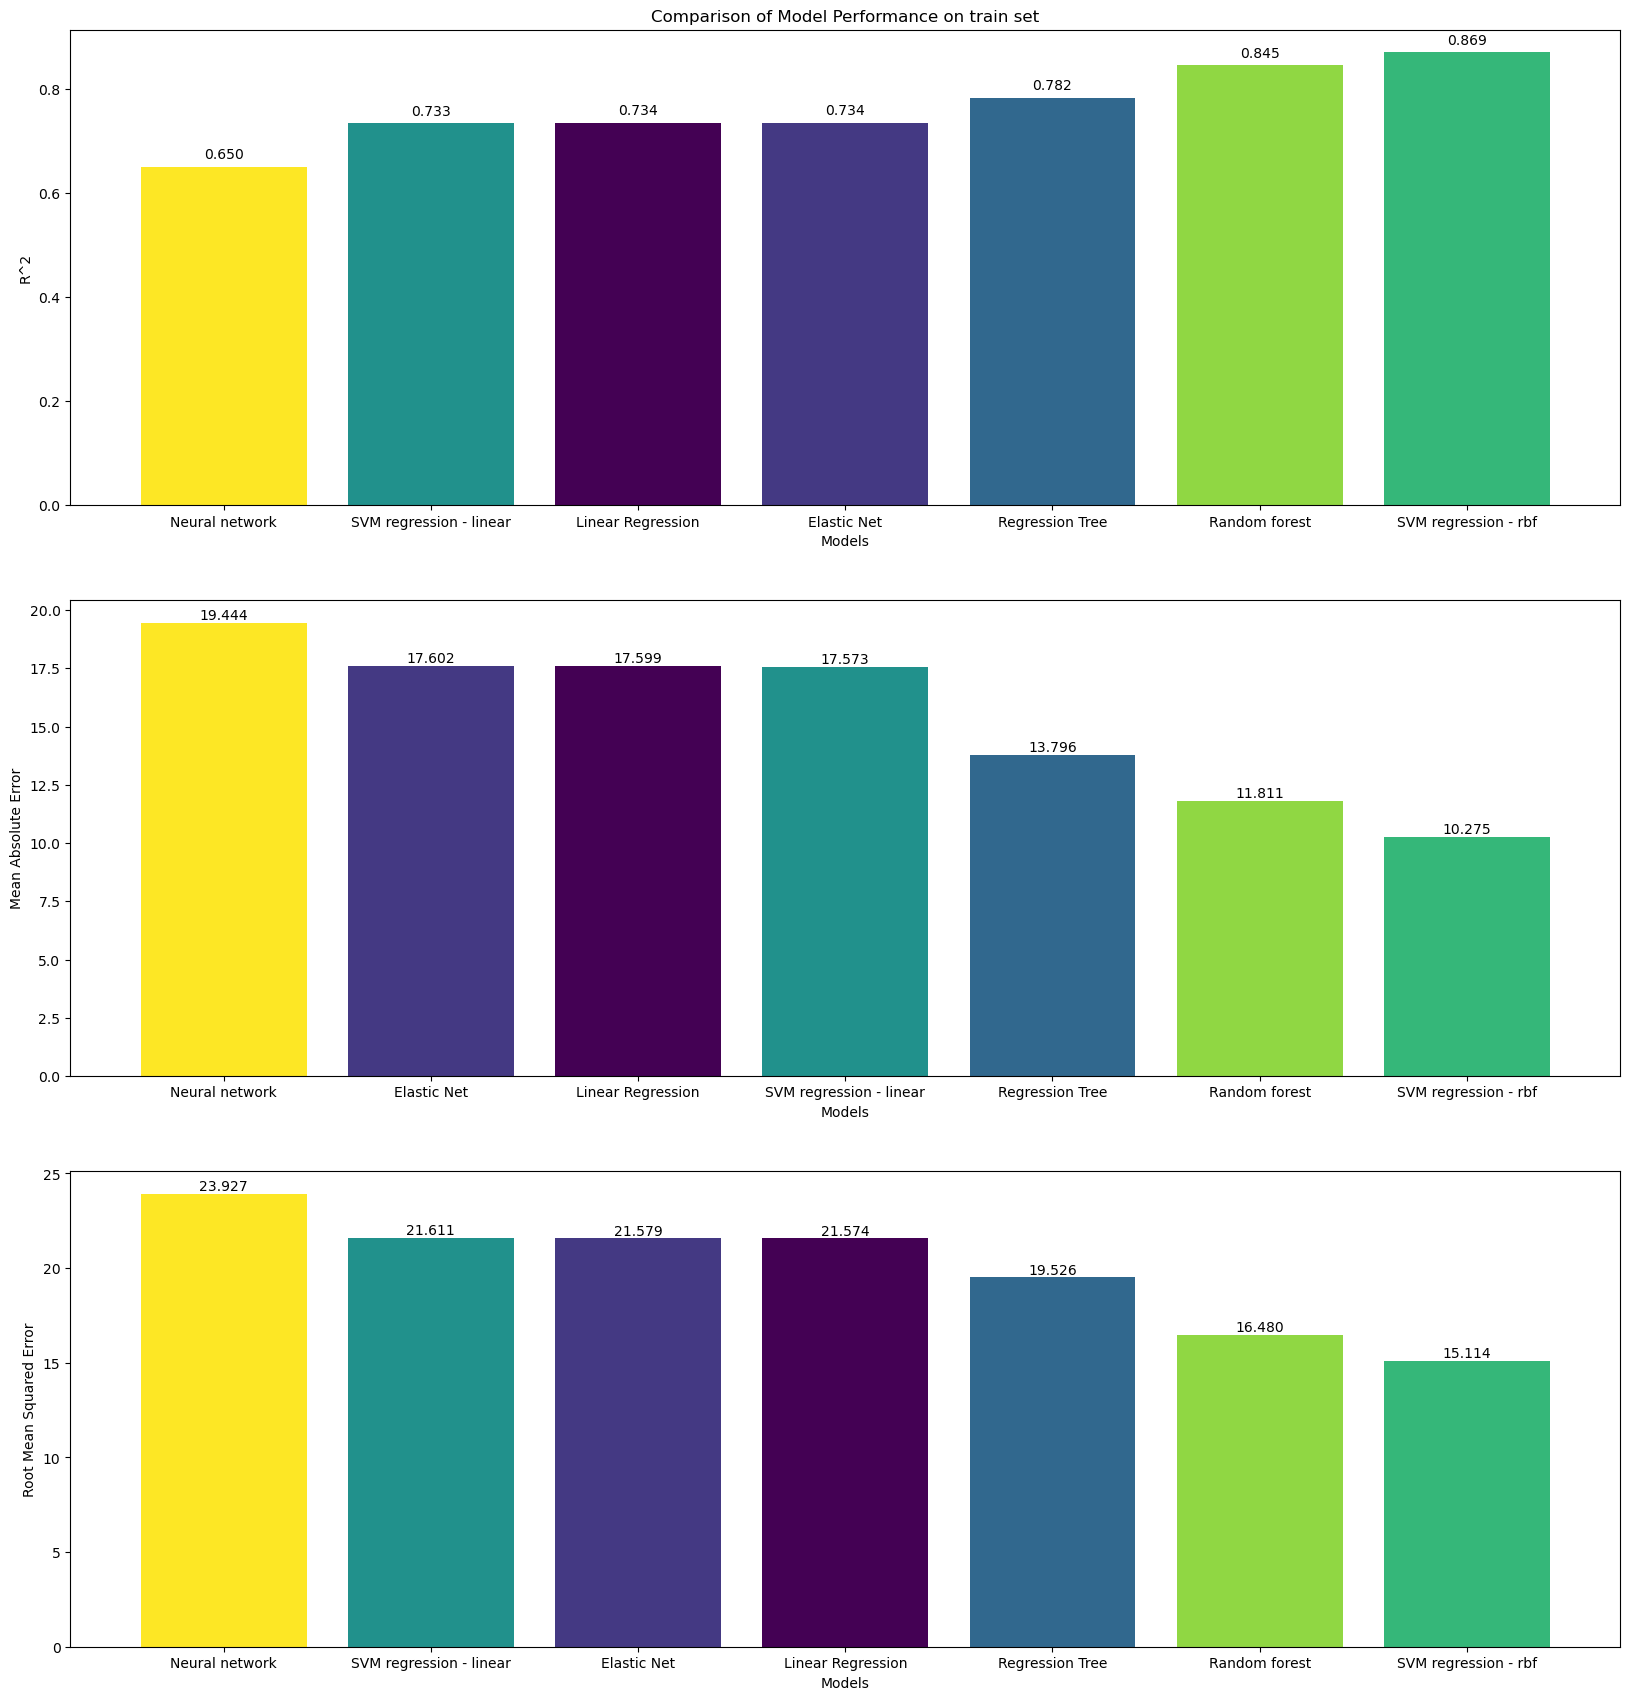
\includegraphics[width=0.8\textwidth]{images/train_model_comparison.png}
    \caption{Comparison of Model Performance on train set.}
    \label{fig:train_model}
\end{figure}

The Random Forest model exhibited the best overall performance across the test sets and the second best performance on the train set, achieving high R² values (0.845 on training and 0.814 on test) and the lowest errors (MAE: 11.011 on training and 12.904 on test; RMSE: 16.480 on training and 17.742 on test). This suggests that Random Forests are highly effective at capturing the complex relationships in the data that are highly non-linear. 

\begin{figure}[H]
    \centering
    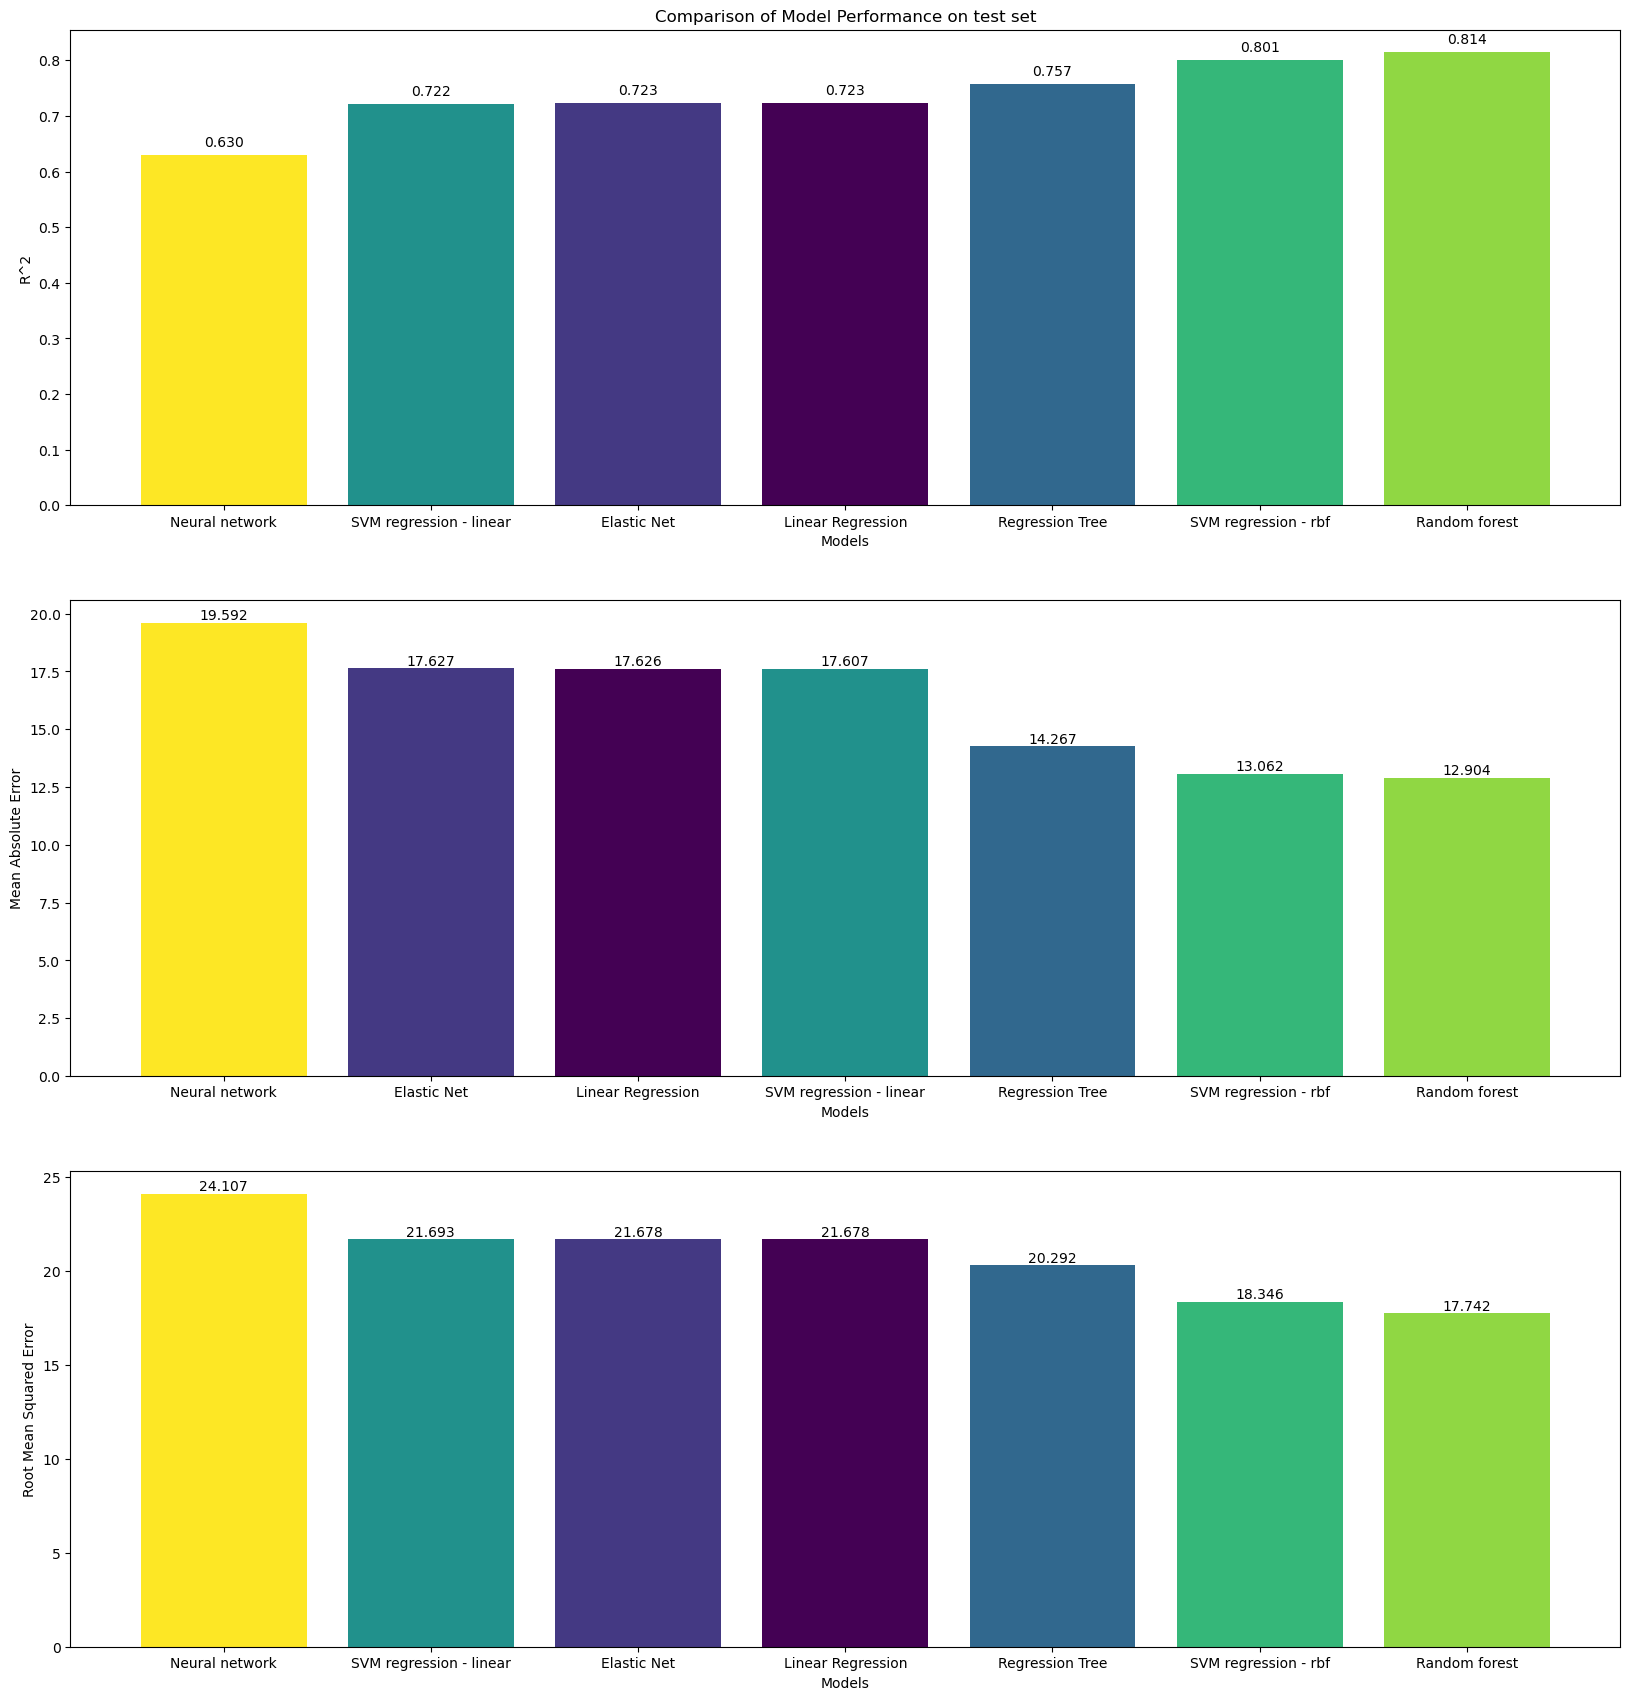
\includegraphics[width=0.8\textwidth]{images/test_model_comparison.png}
    \caption{Comparison of Model Performance on test set.}
    \label{fig:test_model}
\end{figure}

The SVM with RBF kernel also performed exceptionally well, particularly in capturing non-linear relationships, as evidenced by its highest R² value on the train dataset and the second highest score in the test dataset (0.869 on training and 0.801 on test) and low errors (MAE: 10.275 on training and 13.062 on test; RMSE: 15.114 on training and 18.346 on test). This model's ability to handle non-linearity makes it a strong candidate for RUL prediction in turbofan engines.

Linear models, including Linear Regression and Elastic Net, performed moderately well, with similar R² values around 0.723 on the test set and MAE/RMSE around 17.6/21.7, indicating that while they capture some relationships in the data, their simplicity limits their predictive power compared to more complex models. Linear and Elastic Net regression have similar values, that shows that the regularization parameters didn't affect much the Linear model.

Neural Networks, despite their flexibility, did not perform as well as expected, likely due to the limited size and complexity of our dataset. The Neural Network model had the lowest R² values (0.650 on training and 0.630 on test) and higher errors compared to Random Forest and SVM models.


Regression Trees provided a good balance between simplicity and performance, with better results than linear models but not as strong as Random Forest or SVM with RBF kernel.

\subsection{Reflections on the Results}
Pre-processing the dataset is effective because by applying feature selection and correlation analysis, data cleaning, and data smoothing steps on the dataset, it ensured that the models used the most relevant features for prediction. It also reduced noise and improved accuracy of the model.

Potential Improvements could be to apply advanced feature engineering, removing and cleaning out anomalous readings would improve the performance of the model. 

Hyperparameter tuning, especially for non-linear complex models like Random Forests and SVMs led to improvement in results.


\section{Conclusions}

Our study demonstrates that for predicting the remaining useful life of turbofan engines, ensemble methods like Random Forests and sophisticated models like SVM with RBF kernel offer superior performance over simpler models such as Linear Regression and Elastic Net. The Random Forest model based on the achieved result shows high accuracy and robustness, making it a highly suitable choice for this task. These high-performance numbers were achieved mainly with max thresholding of RUL with the given number before it started going nonlinear, as explained in figure \ref{fig:rul_cliping_comparison}.

Future work could explore further enhancements such as more detailed hyper-parameters tuning and the integration of more advanced deep learning models, like Recurrent Neural Networks. Additionally, expanding the models with the use of other available sub-datasets with slightly different features, could improve model generalization and accuracy.


\section{Contributions}

The authors Roberto Cialini, Jaka Škerjanc, Riccardo Rossi-Erba, Jan Fiala, and Chisom Okoye all partook and contributed equally to this project.

%%%%%%%%%%%%%%%%%%%%%%%%%%%%%%%%%%%%%%%%%%%%%%%%%%%%%%%%%%%%%%%
% DO NOT EDIT ANYTHING ABOVE THIS LINE
% EXCEPT IF YOU LIKE TO USE ADDITIONAL PACKAGES
%%%%%%%%%%%%%%%%%%%%%%%%%%%%%%%%%%%%%%%%%%%%%%%%%%%%%%%%%%%%%%%

\newpage
\bibliography{mybibfile}

\end{document}